\documentclass[10pt,oneside,makeidx,letter]{uhthesis}
\usepackage[spanish]{babel}
\selectlanguage{spanish}
\usepackage[utf8]{inputenc}
\usepackage{graphicx}
\usepackage{amsfonts}
\usepackage{listings}
\usepackage{lipsum}
\usepackage{hyperref}
\usepackage{amsmath}
\usepackage{url}

\lstset{frame=tb,
	language=python,
	aboveskip=3mm,
	belowskip=3mm,
	showstringspaces=false,
	columns=flexible,
	basicstyle={\small\ttfamily},
	numbers=none,
	numberstyle=\tiny\color{gray},
	commentstyle=\color{gray},
	breaklines=true,
	breakatwhitespace=true,
	tabsize=3
}
\title{Sistema para la gestión de horarios.}
\author{José Carlos Hernández Piñera}
\advisor{Lic. Pedro Quintero Rojas}
\degree{Licenciado en Ciencias de la Computación}
\faculty{Facultad de Matemática y Computación}
\date{Noviembre de 2022}
\logo{Graphics/uhlogo}

%\makenomenclature

\begin{document}
	
	\frontmatter

	\maketitle	
	
	\begin{acknowledgements}
%	Quisiera agradecer, por el apoyo que me han brindado de distintas formas a lo largo de toda la carrera, a las siguientes personas:
%	
%	A mi madre, que no se rindió cuando yo sí lo hice.
%	
%	A mi padre, por apoyarme, a su manera.
%	
%	A mis tíos Rafael y Juana María y mi primo David, que siempre estuvieron ahí para lo que hiciera falta.
%	
%	A José Carlos, Jonathan y Luis Angel. Primer año no hubiese sido lo mismo sin ustedes.
%	
%	A Eziel, quien ha resultado ser un verdadero amigo. 
%	
%	A Gilberto, compañero de mil proyectos, y sobre todo, amigo. También agradezco a su madre, por todo el apoyo y atención que me brindó.	
%	
%	A mis profesores Wilfredo, Idania y Somoza, quienes me trasmitieron valiosas enseñanzas, no sólo de la materia que impartían.
%	
%	A mi tutor Luciano García, por aceptarme como tesista y dedicarme parte de su tiempo y atención.
%	
%	A todos con los que fui injusto y no mencioné pero que de una forma u otra me ayudaron a ser mejor persona.
\end{acknowledgements}
	\begin{opinion}
	La causalidad ha sido desarrollada por los seres pensantes como una forma de explicar y por 
	consiguiente conocer el mundo que lo rodea y actuar transformándolo. Por ello ha sido objeto de estudio a través de la historia del pensamiento humano, habiendo sido objeto de valiosas reflexiones fundamentalmente en el campo de la filosofía. Pero por muchos años continuó siendo	considerada una modalidad cualitativa del pensamiento humano hasta que la llegada de la estadística y algunas deficiencias en el análisis cuantitativo de los datos puso en evidencia la necesidad de desarrollar la causalidad sobre bases cuantitativas como complemento de la correlación y demás procederes estadísticos.
	
	El trabajo de diploma que presenta para su defensa el estudiante Antonio Jesús Otaño Barrera introduce, de manera innovadora, recientes resultados sobre la modelación cuantitativa de la causalidad utilizando específicamente modelos estructurales causales acompañados de una implementación con una interfaz amistosa con la cual es posible experimentar diferentes modalidades de la causalidad.
	 
	Es de señalar la disciplina y el rigor con el que el estudiante enfrentó la tarea sobre un tema que le era totalmente desconocido y como fue satisfaciendo todos los requisitos que le fueron planteados para su realización. Creemos que el estudiante Antonio Jesús Otaño Barrera ha alcanzado el nivel de profesionalidad que exige alcanzar el título de Lic. en Ciencia de la Computación y por tal motivo solicitamos la calificación de Excelente (5) para su trabajo de diploma.
	
	La Habana, 20 de noviembre de 2021.
	
	
\includegraphics[width=100px, height=80px]{./images/opinion.png}
	
	Dr. Luciano García Garrido
	
	Profesor Titular Consultante
	
	Facultad de Matemática y Computación	
	
	Universidad de La Habana, Cuba
	
\end{opinion}
	\begin{spanish_abstract}
%	La estadística tradicional se ocupa principalmente de la asociación entre variables pero no revela información acerca de las relaciones de causalidad entre estas. A partir de estas limitaciones es necesario la construcción de una teoría que formalice matemáticamente los procesos causales. Dicha teoría permitirá modelar situaciones de la vida cotidiana y responder preguntas causales acerca de estas. Un objetivo más ambicioso consiste en la simulación del razonamiento causal humano, el cual se cree que debe ser una pieza fundamental en la construcción de una inteligencia artificial fuerte. En el presente trabajo se presentarán los principales desarrollos recientes de teorías matemático computacionales de la causalidad, con especial énfasis en el trabajo de Judea Pearl, y se proveerá una implementación de un modelo causal capaz de responder distintos tipos de preguntas causales. Por último, se exponen posibles escenarios donde se puede utilizar el programa propuesto.
\end{spanish_abstract}


	\begin{english_abstract}
	Traditional statistics deals mainly with the association between variables but does not reveal information about the causal relationships between them. Based on these limitations, it is necessary to build a theory that mathematically formalizes causal processes. This theory will allow modeling everyday life situations and answering causal questions about them. A more ambitious goal is the simulation of human causal reasoning, which is believed to be a fundamental piece in building strong artificial intelligence. In this paper, the main recent developments of computational mathematical theories of causality will be presented, with special emphasis on the work of Judea Pearl, and an implementation of a causal model capable of answering different types of causal questions will be provided. Finally, possible scenarios are exposed where the proposed program can be used.
\end{english_abstract}

	\tableofcontents
\listoffigures
\listoftables
	
	\mainmatter
	%\chapter*{Introducción}\label{chapter:introduction}
\begin{introduction}
	Desde tiempos de antaño el hombre se ha visto en la necesidad imperiosa de manejar de la manera más adecuada posible sus recursos, no solo para conseguir prolongar la vida de estos, sino además para contar con una aceptada utilización de los mismos. Uno de los principales problemas que aqueja a la sociedad actual es la dificultad que se presenta para garantizar un óptimo manejo de nuestro \textit{tiempo}.
	
	La denominada \textit{gestión del tiempo} hace referencia a la forma en que cada uno organiza y planifica cuánto invierte en actividades específicas; pasar más horas en la empresa no significa ser más eficiente o productivo; por ello, es fundamental una adecuada gestión del horario en el trabajo, lo que permitiría lograr más con menos esfuerzo. Cuando se aprende a administrar mejor el día a día y las labores cotidianas se mejora la capacidad de concentración, lo que trae consigo un mayor enfoque y por tanto una mayor eficiencia. Gestionar el tiempo nos permite realizar las tareas con más rapidez y que la jornada laboral sea más efectiva y se aproveche mejor.
	
	En muchos escenarios cotidianos la planificación de las actividades se realiza solamente de manera irreal, por otro lado, existen ámbitos donde se hace necesario garantizar una manipulación detallada de todo el proceso.
	
	Con la llegada de las tecnologías actuales y la facilidad con que las personas cambian de actividad, el desarrollo de un software que garantice una planificación de nuestra agenda diaria, resulta casi imprescindible.
	
	Un ejemplo claro donde sin duda se comprueba el proceso antes expuesto, es la gestión de las actividades de un centro de estudios y más aún en esta época donde contamos con grandes instituciones universitarias que albergan a cientos de estudiantes con diferentes planes de trabajo y manejan una gran cantidad de recursos y útiles.
	
	Quizá muchos consideren que realizar la labor de confección de un horario para una institución universitaria es algo sencillo, pero cabe destacar que la persona encargada de dicha labor, emplea un valioso tiempo en esto; puesto que hay que preveer que no existan colisiones entre los turnos, los locales, los profesores, además de garantizar que todas las actividades se realicen con la frecuencia que corresponde para garantizar el aceptado desarrollo del proceso de aprendizaje por parte del estudiantado.
	
	Resulta llamativo como un gran número de universidades cubanas hoy en día aún no cuentan con un sistema propio (o de terceros) para realizar las tareas de confección del horario; sino que en la mayoría de los casos usan softwares como \textit{Microsoft Excel} para gestionar el mismo; lo cual, sin lugar a dudas es sumamente ineficiente y genera un esfuerzo extra para la persona que está desarrollando el mismo, quién sin lugar a dudas debe tener otra serie de tareas que requieran de más importancia.
	
	El trabajo en cuestión persigue presentar un software para proporcionar un sistema que permita manejar el sistema de turnos de clases de la \textit{Facultad de Matemática y Computación} de \textit{La Universidad de La Habana}.
	
	\section{Motivación}
	Desde hace poco más de \textbf{X} años en la Facultad de Matemática y Computación se ha venido gestado la idea de presentar un modelo de horario propio que sea capaz de satisfacer las necesidades internas de la misma. Con anterioridad se han realizado otras tesis de diplomas dedicadas a abordar cuestiones más especifícas relacionadas con esta índole; dígase: manejo de restricciones, generación automática de horarios, entre otros aspectos. 
	
	Las herramientas analizadas previamente, que resolvían el problema del horario, en su mayoría presentaban carencias que se consideraron escenciales a la hora de darle solución al asunto que estamos abordando. Dichas carencias se manejaron dentro del software presentado para garantizar que fueran cubiertas y erradicadas en su totalidad.
	
	Los beneficios finales que ofrecerá el software llaman la atención y es sumamente viable tratarlos como aspectos motivadores a la hora de analizar el resultado final. Se contará por ejemplo, con un sistema de restricciones asociado a todas las entidades del sistema y no solo centrado en los turnos de clases y los profesores; aunque es válido notar que casi todas las condiciones impuestas se relacionan con estos campos. 
	
	El software posibilitará también contar con un sistema centralizado, alojado dentro del nodo de la facultad, lo que hará posible que se pueda acceder en tiempo real por todos los estudiantes y los profesores. Además esto hará más factible la distribución y la organización interna de la institución, puesto que cualquier cambio dentro del sistema, puede ser analizado inmediatamente por todos los interesados.
	
	La edición y el mantenimiento del software, también se realizará de manera relativamente sencilla, con esto se garantiza que se pueda adicionar en el futuro cualquier otra funcionalidad que se considere necesaria o que aporte algún beneficio a la universidad. 
	
	Los profesores son considerados usuarios privilegiados dentro de la aplicación, pues se permite que estos interactuen directamente con los turnos y que muestren sin necesidad de ser administradores, sus inconformidades - por medio de las restricciones -  con la distribución presentada.
	
	Para la persona encargada de la creación del horario, un sistema dedicado especialmente a esto, trae consigo una mejora sustancial; pues es posible detectar datos erróneos durante la confección, se puede tener un control detallado de los profesores, así como de la gestión de locales para poder determinar fácilmente cuáles se encuentran disponibles en un momento y espacio determinado.
	
	En muchos casos es necesario obtener aulas vacías, simplemente para dedicarlas a otra actividad o porque se pretenden usar en otro tipo de eventos. En un gran número de casos esto puede traer un trabajo extra para la persona encargada de realizar tal gestión. El sistema propuesto posibilita que tal tarea se realice en cuestiones de segundos y sin esfuerzo alguno, debido a que se proporcionan varias vistas o formas de representar el conjunto de turnos que ofrecen una solucióna al problema que se plantea. La distribución por recursos, cubre tal aspecto; ya que se identifican todos los locales dentro de la facultad y los horarios en que están ocupados o libres los mismos; además empleando los filtros personalizados se puede hacer incluso más sencilla la tarea.

	
	\section{Objetivos}
	Se tiene como \textbf{objetivo general} presentar una aplicación web que cubra las carencias y dificultades que se tienen en la facultad de Matemática y Computación de La Universidad de La Habana con respecto a la gestión, distribución y creación del sistema de horarios. 
	La aplicación debe ser lo más sencilla posible para permitir que todo tipo de usuarios interactúen con ella. Como \textbf{objetivos más específicos}, el sistema deberá:
	\begin{enumerate}
		\item Identificar las colisiones presentes entre los turnos, profesores y locales.
		\item Mostrar diversas vistas que hagan posible el chequeo de los turnos de la manera más productiva posible (vista de locales, diaria, por semanas, mensual).
		\item Visualizar en culquier momento que se considere necesario, no solo el horario completo sino secciones específicas del mismo.
		\item Permitir la generación de archivos en formato \textit{Excel}, para ser exportados, y que cuenten con toda la distribución de los turnos de clase.
		\item Permitir el manejo de restricciones o condiciones impuestas sobre todas las entidades del sistema y refelejar el cumplimiento (o no) de estas en una sección dedicada.
		\item Ofrecer un manejo de los profesores, asignaturas, grupos, locales y demás aspectos relacionados con una institución educacional.
		\item Cubrir el manejo de varias facultades a la vez e incluso, llegado a ser el caso de varias universidades. 
	\end{enumerate}
	
	El presente trabajo se estructura como se detalla a continuación: en el capítulo 2 se mostrará todo lo referente al estado del arte, así como una descripción de los softwares y herramientas previamente analizados, mostrando además la carencia de estos y por consiguiente la necesidad de construir uno propio que cubra las necesidades internas de la facultad. En el capítulo 3 se presenta una descripción más detallada del problema así como el enfoque de solución ofrecido. Por último en el capítulo 4 se describirán todos los detalles de implementación referentes al software presentado.
	
	\section{Convenciones de estilos}

\end{introduction}

	\chapter{Antecedentes}\label{chapter:state_of_the_art} 

Mejorar este capitulo. \\\\ 

El tema del manejo, creación y gestión de un sistema de horarios ha sido abordado por un gran número de personas, en muchos ámbitos diferentes.

\section{Herramientas de gestión}
El ejemplo más concreto que se analizó antes de la creación del presente trabajo fue un sistema desarrollado en 2019 entre un grupo de universidades de América del Norte y Europa: \href{https://www.unitime.org/}{UniTime}. Este sistema ofrece soporte en un gran número de escenarios, dígase por ejemplo la creación de una especie de salas para la planificación de eventos así como el manejo de secciones individuales por estudiantes. Además cuenta con una pequña comunidad que brinda soporte al mismo por lo que se realizan versiones y modificaciones periódicamente.

Otra herramienta que también llamo la atención fue \href{http://www.educaria.es/#horarios2}{Unit}. Este software confecciona automáticamente los horarios del colegio a partir de los criterios pedagógicos que se determinen en el centro. Propone al usuario una serie de alternativas diferentes sobre las que se pueden hacer cambios manuales. Incorpora además otras funcionalidades como la posibilidad de crear horas de entrada y recreos de los alumnos a horarios diferentes, rangos de horas en que los profesores deben impartir clases por contrato, horario óptimo de guardias, planificación de sustituciones o estadísticas, entre otras. Este generador de horarios está completamente integrado en la plataforma de gestión Alexia.

Otro sistema que resaltó entre los revisados fue \href{http://www.iplannerapp.com/}{iPlanner}. Se trata de una lista de tareas que dispone de los ajustes necesarios para elaborar y organizar un itinerario escolar con vista diaria, semanal, mensual y anual que, además, incluye un registro de todos los días festivos locales. Los eventos se dividen en categorías e integra herramientas como informes, compatibilidad horaria en otros países y otras basadas en el diseño del horario como diferentes plantillas, colores, símbolos y emoticonos. El usuario contará con la opción de facilitar el horario a otros compañeros o estudiantes a través del correo electrónico o subirlo a la nube. 

La principal cuestión que motivó el desarrollo de un sistema propio de la universidad y la no utilización de estas herramientas que ya existían fue la posibilidad de ofrecer un manejo de restricciones sobre todas las entidades del horario; restricciones que ofrecen un grado de \emph{felicidad} al ser evaluadas y permiten la apreciación por parte del creador del horario de que tan bueno resulta la distribución brindada a los turnos de clases; que viene siendo, en definitiva, el punto central de todas estas herramientas. 

Otros autores manejan en sus sistemas un concepto similar al de \emph{restricción}, pero estas están en todos los casos relacionadas con un profesor y un turno de clase; en cambio en el presente software se permite asociarlas a cualquier entidad definida dentro del sistema, dígase por ejemplo: \emph{local}, \emph{departamento}.

\section{Restricciones}
\label{state_of_art:restrictions}
La idea detrás del manejo e implementación de las restricciones surge a través del trabajo de diploma desarrollado por el estudiante \textit{Joel Rey Travieso Sosa} perteneciente a la Facultad de Matemática y Computación de La Universidad de La Habana.

El análisis y la gestión de las restricciones trajo consigo la clasificación en diferentes grupos:
\begin{itemize}
	\item \textit{Asignación de recursos}: Cuando un recurso debe ser asignado a otro recurso de distinto tipo o a cierto evento
	\item \textit{Asignación de tiempo}: Cuando un evento o recurso debe asignarse a una fecha
	\item \textit{Restricciones de tiempo entre eventos}: Cuando un evento mantiene una relación de tiempo con otro
	\item \textit{Solapamiento de eventos}: Cuando un grupo de eventos comparte un mismo intervalo de tiempo.
	\item \textit{Coherencia entre eventos}: Intentar producir horarios más organizados y convenientes
	\item \textit{Capacidad}: Algunos de los recursos tienen capacidades de uso que no pueden ser vulneradas.
	\item \textit{Continuidad}: Cuando se intenta producir horarios con determinadas características constantes o muy predecibles.
	
\end{itemize}

Además se detectaron cinco grupos fundamentales para clasificar las condiciones o requerimientos del problema:
\begin{itemize}
	\item \textit{Restricciones unarias}: aquellas que involucran un sólo evento, como por ejemplo, las clases de un curso no pueden ser programadas un día lunes.
	\item \textit{Restricciones binarias}: aquellas que involucran dos eventos. Un ejemplo típico son las restricciones de topes de horarios para un curso que requiere un mismo recurso: profesor, sala de clases, etc
	\item \textit {Restricciones de capacidad}: las que se imponen al asignar cursos a salas de clase con capacidad suficiente.
	\item \textit{Restricciones de separación de eventos}:  aquellas que requieren que las actividades estén separadas o siguiendo algún patrón en el tiempo. Algunos ejemplos son las impuestas por políticas de la institución de respetar asignaciones de horarios en patrones predefinidos o las condiciones de no existencia de horas intermedias vacías.
	\item \textit{Restricciones asociadas a los  agentes}: las limitaciones en los horarios asignados para cumplir con las preferencias de los profesores.
\end{itemize}

En la implementación que se ofrece se manejan 4 tipos de restricciones fundamentales, que cubren la descripción antes mencionada.
\begin{itemize}
	\item Restricción de requerimiento de cuenta simple.
	\item Restricción de requerimiento de cuenta de condiciones.
	\item Restricción de requerimiento de distribución de atributos.
	\item Restricción de requerimiento relacional.
\end{itemize}
En los capítulos siguientes se ofrecerá una explicación más detallada de todo los relacionado con estas condiciones impuestas sobre el sistema así como la adecuada definición y formulación de todos los conceptos antes expuestos.

\section{Tecnologías}

Mejorar esto. \\\\

Para la confección del sistema se analizaron diversos escenarios para considerar el que propiciara la obtención de un mejor producto y a la vez que se contara con los conocimientos suficientes en el área para obtener los mejores resultados. 

El sistema está desarrollado en \textit{NestJS} (framework de NodeJS), usando \textit{VueJS} para el frontend y \textit{PostgreSQL} par el manejo de la base de datos.

En el capítulo \ref{cap:implementation_details} dedicado a los detalles de implementación se ofrecerá una explicación más en detalles del porqué de la selección y las bondades que ofrecen las tecnologías empleadas.

%\section{Definiciones previas}
%Los modelos que se estudiarán en esta tesis tendrán como estructura subyacente un grafo dirigido y acíclico (DAG) \ref{fig:dag}.
%
%\begin{figure}[h!]
%	\centering
%	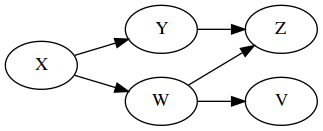
\includegraphics[width=0.5\linewidth]{images/Chapter 2/dag}
%	\caption{Grafo dirigido y acíclico(DAG)}
%	\label{fig:dag}
%\end{figure}
%
%Denotaremos las variables aleatorias con letras mayúsculas ($X$, $Y$, $Z$). A su vez los valores que estas pueden tomar se denotarán con letras minúsculas ($x$, $y$, $z$). Al conjunto de valores que puede tomar una variable $X$ se le denotará $Val(X)$. Para referirnos a un conjunto de variables aleatorias se utilizarán letras mayúsculas en negritas ($\textbf{X},\textbf{Y}$) y para denotar asignaciones a estos conjuntos se emplearán letras minúsculas en negritas ($\textbf{x}$, $\textbf{y}$). Por último, el conjunto de todas las asignaciones que puede darse a un conjunto de variables aleatorias $\textbf{X}$ se denota como $Val(\textbf{X})$.
%
%De especial interés es la Fórmula de Bayes, que permite obtener el valor de la probabilidad condicional $P(X \mid Y)$ a partir del conocimiento previo de $P(Y \mid X)$: 
%
%\begin{theorem}[Fórmula de Bayes]
%	Sean $X$, $Y$ dos variables aleatorias. Entonces la probabilidad condicional $P(X \mid Y)$ se puede calcular como:
%	\[ P(X \mid Y) = \frac{P(Y \mid X ) \cdot P(X)}{P(Y)}  \]
%\end{theorem}
%
%La Ley de Probabilidad Total expresa la distribución de una variable en base a la probabilidad condicional respecto a otra variable:
%\begin{theorem}[Ley de Probabilidad Total]	
%	\[ P(X=x) = \sum_{y} P(X=x \mid Y=y)P(Y=y)\]
%\end{theorem}
%Esta también puede ser aplicada al caso de la probabilidad condicional:
%\[P(X=x \mid Y=y) = \sum_{z}P(X=x \mid Y=y,Z=z)P(Z=z \mid Y=y)\]
%
%La regla de la cadena define la probabilidad conjunta de un conjunto de variables en términos de la probabilidad condicional: 
%\begin{theorem}[Regla de la cadena]
%	Sean $X_1, X_2, ..., X_n$ un conjunto de variables aleatorias. Entonces se cumple que:
%	\[P(X_1,X_2,...,X_n)=P(X_1 \mid X_2,...,X_n)P(X_2 \mid X_3,...,X_n)...P(X_{n-1} \mid X_n)P(X_n)\]
%\end{theorem}
%
%\section{Independencia}
%La teoría de la independencia es fundamental en los modelos gráficos probabilistas. Estos son construidos a partir de las relaciones de independencia que se establecen entre las variables. 
%
%\begin{dfn}[Independencia]
%	Sean las variables aleatorias $X$, $Y$. Se dice que $X$ es independiente (marginalmente)(incondicionalmente) de $Y$ y se denota $X \indep Y$ si $P(X \mid Y) = P(X)$ o si $P(Y)=0$
%\end{dfn}
%Una definición alternativa podría ser:
%\begin{prop}
%	$X \indep Y \Longleftrightarrow P(X,Y)=P(X)P(Y)$
%\end{prop}
%
%En ocasiones dos variables no son independientes por sí solas pero sí lo son a través de una tercera variable. El concepto de independencia condicional recoge estos casos.
%
%\begin{dfn}[Independencia condicional]
%	Sean $X$,$Y$,$Z$ variables aleatorias. Se dice que $X$ es condicionalmente independiente de $Y$ dado $Z$ y se denota $\CondIndep{X}{Y}{Z}$ si $P(X \mid Y,Z)=P(X \mid Z)$ o si $P(Y,Z)=0, \forall x \in Val(X)$.
%\end{dfn}
%
%Similarmente al caso de la independencia marginal, se puede brindar una definición alternativa para la independencia condicional:
%
%\begin{prop}
%	$\CondIndep{X}{Y}{Z} \Longleftrightarrow P(X,Y \mid Z)=P(X \mid Z)P(Y \mid Z)$
%\end{prop}
%
%La independencia condicional satisface un conjunto de propiedades que resultan útiles:	
%\begin{itemize}
%	\item \textbf{Simetría}: $\CondIndep{X}{Y}{Z} \Longrightarrow \CondIndep{Y}{X}{Z}$
%	
%	\item \textbf{Descomposición}: $\CondIndep{X}{Y,W}{Z} \Longrightarrow \CondIndep{X}{Y}{Z}$
%	
%	\item \textbf{Unión débil}: $\CondIndep{X}{Y,W}{Z} \Longrightarrow \CondIndep{X}{Y}{Z,W}$		
%	
%	\item \textbf{Contracción}: $\CondIndep{X}{W}{Z,Y} \& \CondIndep{X}{Y}{Z} \Longrightarrow \CondIndep{X}{Y,W}{Z}$
%	
%\end{itemize}
%\begin{dfn}
%	Una distribución $P$ sobre una variable $X$ se dice que es positiva si para todo $x \in \text{Val(X)}$ se cumple que $P(X=x) > 0$
%\end{dfn}
%\begin{itemize}
%	\item \textbf{Intersección}: Si $P(X)$, $P(Y)$, $P(W)$ y $P(Z)$ son positivas:
%	\[ \CondIndep{X}{Y}{Z,W} \logicand \CondIndep{X}{W}{Z,Y} \Longrightarrow \CondIndep{X}{Y,W}{Z} \]
%\end{itemize}
%
%Los conceptos y propiedades vistos hasta el momento pueden extenderse a conjuntos de variables aleatorias.
%
%\subsection{Independencia condicional en modelos gráficos probabilistas}
%Existen tres tipos de conexiones en los modelos gráficos probabilistas que juegan un papel importante en el análisis de la independencia condicional. Sean $X, Y, Z$ tres variables cualesquiera. Una \textit{cadena} consiste en una conexión del tipo $X \rightarrow Y \rightarrow Z$(Figura \ref{fig:chain}). Una \textit{causa común} consiste en una conexión del tipo $Y \leftarrow X \rightarrow Z$(Figura \ref{fig:fork}). Por último, un \textit{efecto común} es una conexión del tipo $X \rightarrow Z \leftarrow Y$(Figura \ref{fig:collider}).
%
%\begin{figure}[h!]
%	\centering		
%	\begin{subfigure}{\linewidth}
%		\centering
%		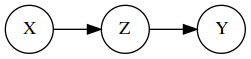
\includegraphics[width=0.40\linewidth]{./images/Chapter 2/chain.png}
%		\subcaption{cadena}
%		\label{fig:chain}
%	\end{subfigure}
%	\begin{subfigure}{0.40\linewidth}
%		\centering
%		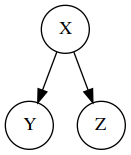
\includegraphics[width=0.5\linewidth]{./images/Chapter 2/fork.png}		
%		\subcaption{causa común}
%		\label{fig:fork}
%	\end{subfigure}
%	\begin{subfigure}{0.40\linewidth}
%		\centering
%		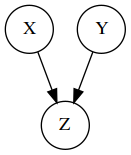
\includegraphics[width=0.5\linewidth]{./images/Chapter 2/collider.png}
%		\subcaption{efecto común}
%		\label{fig:collider}
%	\end{subfigure}		
%	\caption{Tipos de conexiones en un modelo gráfico probabilista}
%	\label{fig:connections}
%\end{figure}
%
%A partir de estas definiciones es posible establecer tres reglas para la determinación de las independencias condicionales en un modelo gráfico probabilista:
%
%\begin{rl}[Independencia condicional en cadenas]\label{rule:chain}
%	Dos variables $X$ y $Y$ son condicionalmente independientes dado \textbf{Z}, si existe un solo camino unidireccional entre $X$ y $Y$, y \textbf{Z} es cualquier conjunto de variables que intercepta ese camino.
%\end{rl}
%
%\begin{rl}[Independencia condicional en causas comunes]
%	Si una variable $X$ es un ancestro común de las variables $Y$ y $Z$, y hay solo
%	un camino entre $Y$ y $Z$, entonces $Y$ y $Z$ son condicionalmente independientes
%	dado $X$.	
%\end{rl}
%
%\begin{rl}[Independencia condicional en efectos comunes]
%	Si una variable $Z$ es descendiente de dos variables $X$ y $Y$, y existe un solo camino entre $X$ y $Y$, entonces $X$ y $Y$ son marginalmente independientes pero condicionalmente dependientes dado $Z$ o cualquiera de los descendientes de $Z$
%\end{rl}
%
%En la figura \ref{fig:chain-indep} si tomamos  $\textbf{Z}=\{V,Z\}$ y aplicamos la Regla \ref{rule:chain}, se cumple que $\CondIndep{X}{Y}{\textbf{Z}}$. A su vez, en la figura \ref{fig:fork-indep}, donde existe la causa común $Y \leftarrow X \rightarrow W$ si conocemos el valor de $X$ entonces se cumple que $\CondIndep{Y}{Z}{\textbf{X}}$. Por último, en la figura  \ref{fig:collider-indep}, tenemos el efecto común $X \rightarrow Z \leftarrow Y$, por tanto las variables $X$ y $Y$ son marginalmente independientes pero condicionalmente dependientes dado $Z$ o $W$.
%
%\begin{figure}[h!]
%	\centering		
%	\begin{subfigure}{\linewidth}
%		\centering
%		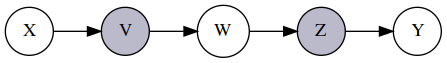
\includegraphics[width=0.6\linewidth]{./images/Chapter 2/chain-indep.png}
%		\subcaption{$\CondIndep{X}{Y}{V,Z}$}
%		\label{fig:chain-indep}
%	\end{subfigure}
%	\begin{subfigure}{0.40\linewidth}
%		\centering
%		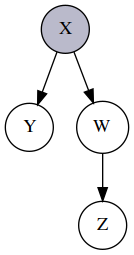
\includegraphics[width=0.5\linewidth]{./images/Chapter 2/fork-indep.png}		
%		\subcaption{$\CondIndep{Y}{Z}{X}$}
%		\label{fig:fork-indep}
%	\end{subfigure}
%	\begin{subfigure}{0.40\linewidth}
%		\centering
%		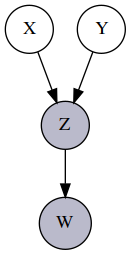
\includegraphics[width=0.5\linewidth]{./images/Chapter 2/collider-indep.png}
%		\subcaption{$X \indep Y$}
%		\label{fig:collider-indep}
%	\end{subfigure}		
%	\caption{
%		Relaciones de independencia en modelos gráficos probabilistas.
%	}
%	\label{fig:connections-indep}
%\end{figure}
%
%\begin{dfn}
%	Un camino $p$ está bloqueado por un conjunto de nodos $\textbf{Z}$ si y solo si:
%	\begin{enumerate}
%		\item $p$ contiene una cadena de nodos $A \rightarrow B \rightarrow C$ o una causa común $A \leftarrow B \rightarrow C$ tal que $B \in \textbf{Z}$.
%		\item $p$ contiene un efecto común $A \rightarrow B \leftarrow C$ tal que ni $B$ ni ninguno de sus descendientes pertenece a $\textbf{Z}$.
%	\end{enumerate}
%\end{dfn}
%
%\begin{dfn}[d-separación]
%	Si $Z$ bloquea todo camino entre $X$ y $Y$ entonces $X$ y $Y$ están d-separados condicionado a $\textbf{Z}$, y por tanto independientes condicionado a $Z$. En caso contrario se dice que están d-conectados.
%\end{dfn}
%En la figura \ref{fig:d-sep}, se cumple que $A$ esta d-separado de $F$ condicionado a $\textbf{Z}=\{B,C\}$:
%\begin{itemize}
%	\item El camino $A \rightarrow B \rightarrow F$ es una cadena y $B \in \textbf{Z}$, por tanto está bloqueado.
%	\item El camino $A \leftarrow C \rightarrow F$ es una causa común y $C \in \textbf{Z}$, por tanto está bloqueado.
%	\item El camino $A \rightarrow D \leftarrow F$ es un efecto común y no contiene ningún nodo que pertenezca a $\textbf{B}$, por lo que también está bloqueado.
%\end{itemize}
%\begin{figure}[h!]
%	\centering
%	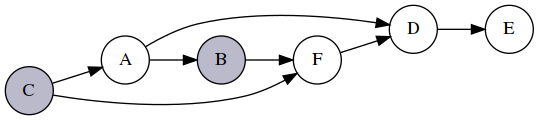
\includegraphics[width=0.8\linewidth]{./images/Chapter 2/d-separation.png}
%	\caption{Ejemplo de d-separación}
%	\label{fig:d-sep}
%\end{figure}	
%
%\section{Redes bayesianas}
%El modelo probabilista que se deriva directamente de la teoría es la distribución de probabilidad conjunta (DPC). Sin embargo, el uso de la DPC conlleva un costo computacional que lo hace impracticable para los problemas reales. Por poner un ejemplo, si se dispone de $n$ variables binarias, la DPC tendría un total de $2^n$ entradas. A partir de estas limitaciones se hace necesario encontrar un modelo alternativo que represente de manera compacta la DPC.
%
%\begin{dfn}[Red bayesiana]
%	Una red bayesiana es un par ordenado $\langle G,P\rangle$ donde:
%	\begin{itemize}
%		\item $G=\langle V,E \rangle$ es un grafo acíclico y dirigido donde $V$ representa a un conjunto de variables aleatorias $X = \{X_1, X_2, ..., X_n\}$ y $E$ determina las relaciones de dependencia entre dichas variables. Sea $Pa_{X_i}$ el conjunto de los nodos padres de $X_i$ en $G$ y $NoDesc_{X_i}$ el conjunto de los nodos que no descienden de $X_i$ en $G$. Entonces para toda variable $X_i$ de $G$ se cumple que: \[\CondIndep{X_i}{NoDesc_{X_i}}{Pa_{X_i}}\]
%		Esta propiedad es llamada la \textit{condición local de Markov}.
%		
%		\item $P$ es una distribución de probabilidad sobre las variables $X_1, X_2, ..., X_n$ que factoriza sobre $G$:
%		\[ P(X_1,X_2,...,X_n)=\prod^{n}_{i=1}P(X_i \mid Pa_{X_i}) \]
%	\end{itemize}
%\end{dfn}
%
%Las redes bayesianas \{pearl1985bayesian} utilizan las relaciones de independencia condicional entre las variables para obtener una representación compacta de la DPC.
%
%Consideremos el caso de una red bayesiana que se usa para modelar el comportamiento de la enfermedad en un paciente (figura \ref{fig:bn-example}). Las variables tenidas en cuenta son: la temperatura del paciente($T$), si este presenta dolor de cabeza($D$), la presencia de la enfermedad en el paciente($E$), la edad ($X$) y el grado de gravedad de la enfermedad($G$).	
%
%\begin{figure}[h!]
%	\centering
%	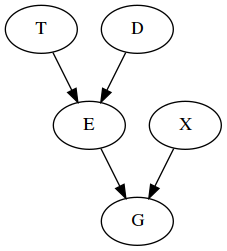
\includegraphics[width=0.3\linewidth]{./images/Chapter 2/bn-example.png}
%	\caption{Una red bayesiana que modela el comportamiento de la enfermedad en un paciente}
%	\label{fig:bn-example}
%\end{figure}
%
%Cada nodo $X_i$ debe almacenar la distribución de probabilidad $P(X_i \mid Pa_{X_i})$. Por ejemplo, si $T$ toma los valores $t_1$ y $t_0$ que indican si tiene o no fiebre, $D$ toma los valores $d_1$ y $d_0$ que indican si tiene o no dolor de cabeza y $E$ toma los valores $e_1$ y $e_0$ que indican si el paciente tiene o no la enfermedad, entonces una posible distribución de probabilidad para $P(E \mid T,D)$ podría ser:
%
%\begin{center}
%	\begin{tabular}{|c|c|c|}
%		\hline 
%		& $e_0$ & $e_1$ \\ 
%		\hline 
%		$t_0,d_0$ & 0.85 & 0.15 \\ 
%		\hline 
%		$t_0,d_1$ & 0.7 & 0.3 \\ 
%		\hline 
%		$t_1,d_0$ & 0.4 & 0.6 \\ 
%		\hline 
%		$t_1,d_1$ & 0.2 & 0.8 \\ 
%		\hline 
%	\end{tabular}		
%\end{center}
%
%\subsection{Inferencia}
%% Several researchers have studied this application, which
%% has been proven to be NP-Hard [16]. An important result
%% is that this complexity can be managed by bounding the
%% treewidth, a measure of the tree-likeness of the graph. The
%% treewidth is defined as the size of the largest clique in a
%% chordal completion of the graph. Modern exact inference
%% algorithms have worst-case time complexity exponential in
%% the treewidth of the underlying graph
%Existen dos tipos principales de inferencia en redes bayesianas: la \textit{actualización de creencias}, también llamada \textit{inferencia probabilística} y la \textit{revisión de creencias}, también llamada \textit{explicación MAP}\cite{10.5555/534975} \cite{guo2002survey}.	La \textit{actualización de creencias} consiste en determinar la distribución conjunta de un conjunto \textbf{X} de variables de la red a partir de un conjunto de evidencias \textbf{E}, determinada por la expresión $P(\textbf{X} \mid \textbf{E})$. La \textit{revisión de creencias} consiste en obtener la configuración más probable de las variables en un conjunto \textbf{X} de variables de la red dado un conjunto de observaciones \textbf{E}. Es decir, se desea obtener el valor de la expresión: $arg$ $max_{\textbf{X}}\{P(\textbf{X}\mid \textbf{E}=\textbf{e})\}$, que indica una asigación $\{X_1=x_1,X_2=x_2,...,X_n=x_n\}$ tal que no exista ninguna otra asignación con mayor probabilidad.
%
%A su vez los algoritmos de inferencia se clasifican en dos grandes categorías: inferencia exacta e inferencia aproximada. 	La inferencia probabilística exacta en general ha sido catalogada como un problema NP-duro por Cooper \cite{COOPER1990393}. La inferencia probabilística aproximada también fue clasificada como NP-duro por Dagum y Luby \cite{DAGUM1993141}. En 1994, Shimony demostró que la revisión de creencias exacta era NP-duro \cite{SHIMONY1994399} y posteriormente en 1998 Abdelbar y Hedetniemi demostraron que la revisón de creencias aproximada también era NP-duro \cite{ABDELBAR199821}.
%
%\subsubsection{Inferencia exacta}
%\label{subsec:exact-inference}			
%En los 80, Pearl publicó un algoritmo que resolvía la inferencia exacta en tiempo polinomial respecto al número de nodos en redes individualmente conectadas \cite{PEARL1986241}. Pearl además publicó un algoritmo para redes con conexiones múltiples en el que transformaba la red en una con conexiones individuales y aplicaba el algoritmo anterior. Sin embargo, el proceso de transformación de la red es un problema NP-completo.
%
%El algoritmo de propagación de inferencia exacta más famoso es el \textit{algoritmo de propagación en árbol de cliques} propuesto por Lauritzen y Spiegelhalter \cite{lauritzen1988local}. También es llamado el \textit{algoritmo de clustering} o \textit{propagación de creencias}. El algoritmo construye el árbol de cliques mediante la triangulación del grafo moral correspondiente al grafo no dirigido subyacente en la red y luego realiza propagación de mensajes en el árbol de cliques. El algoritmo de propagación en árbol de cliques es eficiente en redes esparcidas pero puede ser extremadamente lento en redes densas. En general, se comporta exponencial con respecto al tamaño del clique más grande del grafo moral triangulado.
%
%El algoritmo de \textit{eliminación de variables}(VE)\cite{zhang1994simple} consiste en ir eliminando otras variables una por una e ir sumándolas. La complejidad del algoritmo se mide por el número de sumas y multiplicaciones que se realizan. Una eliminación óptima de las variables conduce a la menor complejidad, pero el problema de hallar una eliminación óptima es NP-completo.
%
%El algoritmo de \textit{Inversión de arcos / reducción de nodos} de Shachter \cite{SHACHTER1990173} \cite{HENRION1990129} aplica una serie de operadores a la red, que invierten la orientación de las aristas usando la regla de Bayes y terminan reduciendo la red al conjunto de nodos que representan a las variables consultadas con los nodos de la evidencia como sus predecesores.
%
%La \textit{inferencia probabilística simbólica}(SPI) ve a la inferencia probabilística como un problema de optimización combinatorio: encontrar una factorización óptima dado un conjunto de distribuciones de probabilidad \cite{LI199455}.
%
%\subsubsection{Inferencia aproximada}
%
%Los algoritmos de simulación estocástica, también llamados muestreo estocástico o algoritmos de Monte Carlo, son los algoritmos de inferencia aproximada más conocidos. Generan un conjunto de muestras seleccionadas al azar o instanciaciones de la red de acuerdo a las tablas de probabilidad condicional del modelo y después estiman las probabilidades de las variables de la consulta por la frecuencia de apariciones en la muestra. La precisión depende de la cantidad de muestras independientemente de la estructura de la red. Pueden ser divididos en dos tipos: \textit{algoritmos de muestreo por importancia} y \textit{Métodos de Monte Carlo con Cadenas de Markov} \cite{guo2002survey}.
%
%Los \textit{métodos de simplificación de modelos} simplifican el modelo hasta que sea factible utilizar un algoritmo de inferencia exacta. Algunos simplifican el modelo eliminado probabilidades pequeñas o consideradas irrelevantes \cite{jensen2013approximations}. Otros involucran la eliminación de arcos \cite{van1997approximating} o de dependencias débiles \cite{kjaerulff1994reduction}. El \textit{algoritmo de espacio de estados} reduce la cardinalidad de las tablas de probabilidad condicional para simplificar el modelo \cite{wellman1994state}.
%
%Los \textit{métodos basados en búsqueda} asumen que una fracción relativamente pequeña del espacio de probabilidad conjunta contiene la mayoría de la masa de probabilidad. Estos algoritmos buscan las instanciaciones de mayor probabilidad y las usan para obtener una aproximación razonable. Entre los más relevantes se encuentran el método de búsqueda \textit{Top-N} de Henrion \cite{henrion1991search} y la variante de búsqueda de Poole usando \textquotedblleft conflictos\textquotedblright \cite{poole1993use, poole1996probabilistic}.
%
%\section{Modelos causales estructurales}
%Las redes bayesianas modelan las dependencias entre las variables pero no nos dicen nada acerca de las relaciones de causalidad entre estas. Una arista de $X$ hacia $Y$ en el DAG de una red bayesiana no implica que $X$ cause a $Y$, sino que existe correlación entre ambas. Para modelar estas relaciones de causalidad es necesario un modelo que defina explícitamente las mismas.
%\begin{dfn}[Modelo Causal Estructural]
%	Un \textit{modelo causal estructural}(SCM) consiste en una tupla $\langle U, V, F\rangle$ donde:
%	\begin{itemize}
%		\item  $U$ es un conjunto de variables llamadas exógenas, términos de error o factores omitidos y representan factores externos al modelo.
%		\item $V$ es un conjunto de variables llamadas endógenas cuyos valores están determinados a partir de factores dentro del modelo.
%		\item $F$ es un conjunto de funciones que determinan los valores de las variables de $V$ a partir de los valores de un subconjunto de variables de $U \cup V$.
%	\end{itemize}
%\end{dfn}
%
%A partir de una asignación completa a las variables de $U$ es posible determinar perfectamente el valor de todas las variables de $V$ mediante las funciones de $F$. Cada variable $U_i \in U$ tiene asignada una distribución de probabilidad $P(U_i)$. De esta forma se añade no determinismo al modelo.
%
%En el presente trabajo nos limitaremos a los modelos completamente especificados, donde se conocen todos los valores que pueden tomar todas las variables del modelo, así como su función de definición en el caso de las variables endógenas o su distribución de probabilidad en el caso de las exógenas. Se asume además que las variables exógenas son independientes entre sí. Por último, una variable no puede estar definida en términos de sí misma y en general no pueden existir dependencias cíclicas entre las variables.
%
%Cada SCM tiene asociado un grafo dirigido acíclico que representa las relaciones de causalidad entre las variables del modelo. Cada vértice representa una variable del modelo y para cualesquiera dos variables $X$, $Y$ tal que $Y$ depende de $X$, existe una arista en el grafo dirigida del nodo que representa a $X$ hacia el de $Y$. A partir de la relación entre un SCM y su modelo gráfico es posible establecer una definición gráfica de causalidad:
%
%\begin{dfn}
%	Sea $M=\langle U,V,F \rangle$ un SCM y sea $G$ su grafo asociado. Sean las variables $X,Y \in U\cup V$:
%	\begin{itemize}
%		\item $X$ es una causa directa de $Y$ si existe una arista de $X$ hacia $Y$ en $G$.
%		\item $X$ es una causa potencial de $Y$ si $X$ es ancestro de $Y$ en $G$.
%	\end{itemize}
%\end{dfn}
%
%Supongamos que se tiene un circuito lógico de dos entradas($X$, $Y$) unidas por una compuerta AND($Z$) y la salida de esta es negada($W$). Un modelo causal estructural para este ejemplo podría ser el siguiente:
%\begin{model}
%	\[
%	\arraycolsep=10pt
%	\begin{array}{ccc}
%		U = \{X, Y\}&
%		V = \{Z, W\}&
%		F = \{f_z, f_w\}
%	\end{array}
%	\]
%	
%	\begin{center}
%		$P(X=0)=P(X=1)=P(Y=0)=P(Y=1)=0.5$
%		\[
%		\begin{array}{cc}
%			f_z: & Z = X \cdot Y \\ 
%			f_w: & W = 1 - Z
%		\end{array} 
%		\]
%	\end{center}
%\end{model}
%
%En la figura \ref{fig:scm} se muestra el DAG asociado a este modelo, que representa las relaciones de causalidad entre las variables. Se cumple que $X$ es una causa directa de $Z$, y a la vez es una causa potencial de $W$.
%
%\begin{figure}[h!]
%	\centering
%	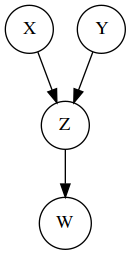
\includegraphics[width=0.2\linewidth]{./images/Chapter 2/pscm-example.png}
%	\caption{Grafo aociado a un modelo causal que representa el comportamiento de un circuito lógico.}
%	\label{fig:scm}
%\end{figure}
%
%Si realizamos las asignaciones $X=1$ y $Y=0$ a las variables de $U$ entonces, mediante las funciones de correspondientes, obtenemos que $Z=0$ y $W=1$.		
%
%\subsection{Relación entre modelos estructurales causales y redes bayesianas}
%\label{secc:scm-bn}
%A partir de un modelo causal estructural es posible obtener una red bayesiana que codifique la información del modelo. De esta forma se preservarán las relaciones de causalidad entre las variables y será posible utilizar una red bayesiana para responder a preguntas causales.
%
%Sea $M=\langle U,V,F \rangle$ un modelo causal estructural. Entonces es posible construir una red bayesiana $N=\langle G,P\rangle$ tal que:
%\begin{itemize}
%	\item $G$ es el modelo gráfico causal de $M$.
%	
%	\item $P'$ es un conjunto de distribuciones de probabilidad condicional $P'(X \mid Pa_X)$, tal que $X \in U \cup V$ y $Pa_X$ denota los padres de $X$ en $G$. Si $X \in U$, entonces $Pa_X = \emptyset$ y $P'(U_i)=P(U_i)$ . En caso de que $X \in V$ entonces, la distribución de probabilidad condicional se define como:
%	
%	\begin{equation*}
%		P'(X=x|Pa_X=x^{\ast}) = 
%		\left\{
%		\begin{array}{ll}
%			1 & \mathrm{si\ } x = F_X(x^{\ast})\\
%			0 & eoc
%		\end{array}
%		\right\}.
%	\end{equation*}
%	donde $F_X \in F$ es la función que define a la variable $X$.
%\end{itemize}
%
%Supongamos que se tiene el modelo:
%
%\begin{model}
%	\[
%	\arraycolsep=10pt
%	\begin{array}{ccc}
%		U = \{X, Y\}&
%		V = \{Z\}&
%		E = \{f_z\}
%	\end{array}
%	\]
%	\begin{center}
%		$f_z: Z = X + Y$
%		\begin{equation*}
%			P(X=x) = 
%			\left\{
%			\begin{array}{ll}
%				0.7 & \mathrm{si\ } x = 1\\
%				0.3 & e.o.c
%			\end{array}
%			\right\}.
%		\end{equation*}
%		
%		\begin{equation*}
%			P(Y=y) = 
%			\left\{
%			\begin{array}{ll}
%				0.2 & \mathrm{si\ } y = 1\\
%				0.8 & e.o.c
%			\end{array}
%			\right\}.
%		\end{equation*}
%	\end{center}
%\end{model}
%
%Entonces es posible construir una red bayesiana cuya estructura sea la representada en el grafo de la figura \ref{fig:scm-to-bn}.
%
%\begin{figure}[h!]
%	\centering
%	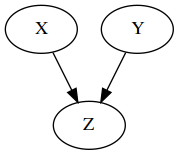
\includegraphics[width=0.3\linewidth]{./images/Chapter 2/scm-to-bn.png}		
%	\caption{Grafo que representa la estructura de una red bayesiana obtenida a partir de un modelo estructural causal probabilístico}
%	\label{fig:scm-to-bn}
%\end{figure}
%
%Por otro lado, asumiendo que $\text{Val}(X)={Val}(Y)=\{0,1\}$ y $\text{Val(Z)=\{0,1,2\}}$, las las de probabilidad asociadas a los nodos se pueden construir siguiendo las reglas descritas anteriormente:
%\begin{center}
%	\begin{tabular}{|c|c|}
%		\hline 
%		$X$ & $P(X)$ \\ 
%		\hline 
%		0 & 0.3 \\ 
%		\hline 
%		1 & 0.7 \\ 
%		\hline 
%	\end{tabular}
%	\quad
%	\begin{tabular}{|c|c|}
%		\hline 
%		$Y$ & $P(Y)$ \\ 
%		\hline 
%		0 & 0.8 \\ 
%		\hline 
%		1 & 0.2 \\ 
%		\hline 
%	\end{tabular}
%	\quad
%	\begin{tabular}{|c|c|c|c|}
%		\hline 
%		$X$ & $Y$ & $Z$ & $P(Z \mid X,Y)$ \\ 
%		\hline 
%		0 & 0 & 0 & 1 \\ 
%		\hline 
%		0 & 0 & 1 & 0 \\ 
%		\hline 
%		0 & 0 & 2 & 0 \\ 
%		\hline 
%		0 & 1 & 0 & 0 \\ 
%		\hline 
%		0 & 1 & 1 & 1 \\ 
%		\hline 
%		0 & 1 & 2 & 0 \\ 
%		\hline 
%		1 & 0 & 0 & 0 \\ 
%		\hline 
%		1 & 0 & 1 & 1 \\ 
%		\hline 
%		1 & 0 & 2 & 0 \\ 
%		\hline 
%		1 & 1 & 0 & 0 \\ 
%		\hline 
%		1 & 1 & 1 & 0 \\ 
%		\hline 
%		1 & 1 & 2 & 1 \\ 
%		\hline 
%	\end{tabular}
%\end{center}
%\section{Intervenciones}
%Una \textit{intervención}, en su variante más simple, consiste en determinar el comportamiento de una variable $Y$ cuando otra variable $X$ es forzada a tomar un valor $x$. El resultado de una intervención está determinado por la expresión $P(Y \mid do(X))$. El operador $do$ indica que la variable $X$ es intervenida.
%
%Es importante recalcar la diferencia que existe entre $P(Y=y \mid X=x)$ y $P(Y=y \mid do(X=x))$. El primero calcula la probabilidad de $Y=y$ a partir de la observación de $X=x$, mientras que el segundo lo hace a partir de una intervención donde $X$ es forzada a tomar el valor $x$. En términos de distribuciones, $P(Y \mid X=x)$ refleja la distribución de $Y$ en individuos cuyo valor de $X$ es $x$, mientras que $P(Y \mid do(X=x))$ refleja la distribución de $Y$ si todos los individuos de la población son forzados a tomar el valor $X=x$.
%
%El operador $do$ descarta los caminos espúreos entre $X$ y $Y$ que distorsionan el efecto real de $X$ sobre $Y$. Un mundo donde $P(X \mid do(Y))$ fuera igual a $P(X \mid Y)$ estaría lleno de paradojas. Por ejemplo, las personas decidiendo no ir al médico reducirían la probabilidad de enfermarse o se eliminarían las estaciones de policía para reducir el número de crímenes.
%
%El experimento aleatorio controlado ha sido la herramienta por excelencia de los estadísticos para calcular los resultados de una intervención. Sin embargo, estos experimentos suelen ser costosos y en ocasiones incluso imposibles en la práctica. Uno de los logros más notables de la teoría de la causalidad ha sido brindar herramientas para simular una intervención sin llegar a realizarla.
%
%La figura \ref{fig:int-ex:a} muestra el grafo de un modelo que define las relaciones de causalidad entre el género($Y$), tomar un medicamento($X$) y la recuperación del paciente($Y$). Se sabe que el género del paciente afecta la recuperación, así como en la decisión de usar o no el medicamento. Supongamos que se quiere medir el efecto del medicamento en la recuperación de un paciente, o sea $P(Y \mid do(X=x))$.
%
%\begin{dfn}[Submodelo]
%	Sea $M$ un SCM, $X \subset V$ y $x$ una asignación de valores a $X$. Se dice que $M_x$ es submodelo de $M$ si $M_x$ contiene las mismas variables de $U$ y $V$, pero el conjunto de funciones $F$ es sustituido por $F_x$, donde:
%	\[ F_x = \{ F_{V_i} \in F: V_i \notin X \} \cup \{X_i=x_i: X_i \in X \} \]  
%\end{dfn}
%
%Es decir, el submodelo $M_x$ de $M$ se obtiene sustituyendo todas las funciones que definen a las variables de $X$ por la asignación $X_i=x_i$ correspondiente. Gráficamente este procedimiento consiste en eliminar todas las aristas que inciden en las variables de $X$, puesto que ya no dependen de ninguna otra variable sino que se les asigna un valor en concreto. La figura \ref{fig:int-ex:b} muestra el submodelo $M_x$ resultante de intervenir la variable $X$ en el modelo $M$ de la figura \ref{fig:int-ex:a}.
%
%Se cumple entonces que $P(Y=y \mid do(X=x))$ es igual a la probabilidad condicional $P_m(Y=y \mid X=x)$ que prevalece en $M_x$. Para calcular esta última probabilidad, es necesario encontrar invariantes entre $P$ y $P_m$. Por un lado, se sabe que $P_m(Z=z) = P(Z=z)$ dado que eliminar la arista $Z \rightarrow X$ en el grafo original no afecta la probabilidad de $Z$ en el grafo resultante. Por otro lado, también se cumple que $P(Y=y \mid X=x, Z=z) = P_m(Y=y \mid X=x,Z=z)$ porque la forma en la que $Y$ responde a $X$ y $Z$ es la misma independientemente de que una de ellas cambie naturalmente o se fije su valor. Por último, $X$ y $Z$ están d-separados y por tanto son independientes en $M_x$, por lo que $P_m(Z=z \mid X=x)=P_m(Z=z)$. Juntando todas estas consideraciones, se tiene que:
%
%\begin{align}
%	P(Y=y \mid & do(X=x))\\
%	&= P_m(Y=y \mid X=x) \quad \text{(por definición)}\\
%	&= \sum_{z}P_m(Y=y \mid X=x,Z=z)P_m(Z=z \mid X=x)\label{adjust-2}\\
%	&= \sum_{z}P_m(Y=y \mid X=x,Z=z)P_m(Z=z)\label{adjust-3}\\
%\end{align}
%La ecuación \ref{adjust-2} es obtenida mediante la Fórmula de la Probabilidad Total. Utilizando las invariantes anteriores, es posible obtener una fórmula para el efecto causal de $X$ en $Y$ en términos de probabilidades preintervención:
%\begin{equation}
%	P(Y=y \mid do(X=x)) = \sum_{z}P(Y=y \mid X=x,Z=z)P(Z=z) 
%\end{equation}
%La fórmula anterior es denominada \textit{fórmula de ajuste} \cite{pearl2016causal}. En este caso se dice también que se está \textquotedblleft ajustando para $Z$\textquotedblright.		
%
%\begin{figure}[h!]
%	\centering
%	\begin{subfigure}[b]{0.48\linewidth}
%		\centering
%		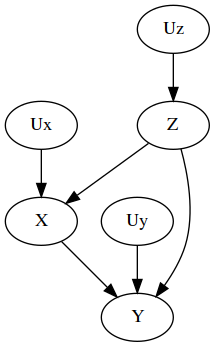
\includegraphics[width=0.65\linewidth]{images/Chapter 2/intervention-example(1).png}
%		\caption{}
%		\label{fig:int-ex:a}
%	\end{subfigure}
%	\begin{subfigure}[b]{0.48\linewidth}
%		\centering
%		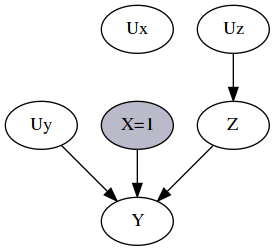
\includegraphics[width=0.8\linewidth]{images/Chapter 2/intervention-example(2).png}
%		\caption{}
%		\label{fig:int-ex:b}
%	\end{subfigure}
%	\caption{Obtención del submodelo resultante de una intervención}
%	\label{fig:int-ex}
%\end{figure}  
%
%La fórmula de ajuste puede ser generalizada si se ajusta con $\textbf{Z}=Pa_X$, el conjunto de los padres de $X$ \cite{pearl2016causal}:
%
%\begin{theorem}[Regla del efecto causal]
%	Sea $G$ un DAG correspondiente a un SCM. El efecto causal de $X$ en $Y$ está determinado por la fórmula:
%	\[ P(Y=y \mid do(X=x)) = \sum_{z} P(Y=y \mid X=x, Pa_X=z)P(Pa_X=z) \]
%	donde $z$ toma todos las posibles combinaciones de valores que pueden tomar los padres de $X$.
%\end{theorem}
%
%A veces interesa medir el efecto de intervenir varias variables. Para ello se utiliza la fórmula del  \textit{producto truncado} o \textit{fórmula-g}:		
%\[P(x_1,x_2,...,x_n \mid do(x))=\prod_{i=1}^{n}P(x_i \mid Pa_{X_i}) \quad \forall X_i: X_i \notin X\]
%La fórmula del producto truncado, como su nombre lo indica, resulta de eliminar los factores que corresponden a las variables intervenidas, de la fórmula de la distribución conjunta. Por ejemplo, supongamos que se tiene la siguiente fórmula de distribución conjunta para un modelo gráfico probabilista:
%\[ P(X,Y,Z,W)=P(X)P(Y \mid X)P(Z \mid X)P(W \mid Y, Z) \]
%Entonces, si se quiere intervenir las variables $Y$ y $Z$, la fórmula del producto truncado queda:
%\[ P(X=x, W=w \mid do(Y=y),do(Z=z)) = P(X)P(W=w \mid Y=y,Z=z)\]
%
%%		\begin{figure}
%%			\centering
%%			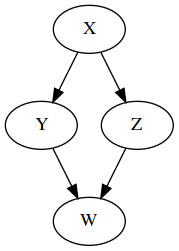
\includegraphics[width=0.4\linewidth]{images/Chapter 2/g-formula(1)}
%%			\caption{}
%%			\label{fig:g-formula}
%%		\end{figure}
%
%\subsection{El criterio de la puerta trasera}
%En ocasiones no es posible ajustar para los padres de una variable porque a pesar de estar representados en el grafo, no se cuenta con suficiente información sobre estos para medirlos. En tales circunstancias es necesario encontrar un conjunto alternativo de variables $\textbf{Z}$ con el que ajustar \cite{pearl2016causal}.
%
%\begin{dfn}[Criterio de la puerta trasera]
%	Dado un par ordenado de variables $(X,Y)$ en un grafo dirigido acíclico $G$, un conjunto de variables $\textbf{Z}$ satisface el criterio de la puerta trasera relativo a $(X,Y)$ si ningún nodo en $\textbf{Z}$ desciende de $X$ y $\textbf{Z}$ bloquea cada camino entre $X$ y $Y$ que contiene una arista que entra a $X$.
%\end{dfn}
%
%Es fácil observar que $Z=Pa_X$, el conjunto de los padres de $X$, satisface el criterio de la puerta trasera. Los caminos de $X$ hacia $Y$ con una arista que incide en $X$ son llamados caminos de puerta trasera de $X$ hacia $Y$.
%
%\begin{theorem}
%	Si un conjunto de variables $\textbf{Z}$ satisface el criterio de la puerta trasera relativo a $(X,Y)$, entonces el efecto causal de $X$ en $Y$ está dado por la fórmula:
%	\[ P(Y=y|do(X=x)) = \sum_{z} P(Y=y|X=x,Z=z)P(Z=z)\]
%\end{theorem}
%
%Supongamos que queremos medir la recuperación de un paciente a partir de una intervención en la que se le suministra un medicamento. En la recuperación del paciente interviene también el peso, y aunque no conocemos su valor, también se sabe que el estatus socio-económico es una causa tanto del medicamento que se le suministra, como del peso del paciente. Se quiere determinar cuán efectivo será el medicamento en la recuperación del paciente(figura \ref{fig:backdoor}).	A pesar de que no conocemos el valor de $Z$, si escogemos $\textbf{Z}=\{W\}$, vemos que este conjunto satisface el criterio de la puerta trasera puesto que bloquea el camino de puerta trasera: $X \leftarrow Z \rightarrow W \rightarrow Y$. Luego la fórmula de ajuste resulta:
%\[ P(Y=y|do(X=x)) = \sum_{w} P(Y=y|X=x,W=w)P(W=w)\]
%
%\begin{figure}[!h]
%	\centering
%	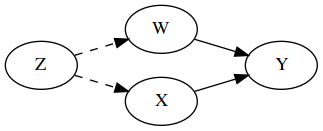
\includegraphics[width=0.35\linewidth]{images/Chapter 2/backdoor-ex.png}
%	\caption{Aplicación del criterio de la puerta trasera}
%	\label{fig:backdoor}
%\end{figure}
%
%Puede que interese identificar el efecto de una intervención no en toda la población sino en un subconjunto de esta que reúna unas características $Z=z$ luego de la intervención. Este es llamado el \textit{efecto z-epecífico}
%
%\begin{dfn}
%	Sean $X,Y$ variables aleatorias y $\textbf{Z}$ un conjunto de variables aleatorias. Se denomina \textit{efecto z-específico} de $X$ en $Y$ al resultado de la expresión: $P(Y=y \mid do(X=x), \textbf{Z}=\textbf{z})$.
%\end{dfn}
%
%\begin{theorem}
%	El efecto z-específico $P(Y=y \mid do(X=x),Z=z)$ es identificado siempre que se pueda encontrar un conjunto de variables $S$ tal que $S \cup Z$ satisface el criterio de la puerta trasera, resultando en la siguiente fórmula de ajuste:
%	\[ P(Y=y \mid do(X=x)) = \sum_{s} P(Y=y \mid X=x, S=s, Z=z)P(S=s)\]
%\end{theorem}
%
%En el modelo de la figura \ref{fig:z-effect(a)} se muestra que el efecto z-específico de $A$ en $E$ no es identificable si se escoge $S=\emptyset$ porque $\{C\}$ no satisface el criterio de la puerta trasera. Sin embargo, en la figura \ref{fig:z-effect(b)} se muestra como escogiendo $S=\{B\}$, entonces este si es identificable, ya que $\{B,C\}$ sí lo satisface. En este caso la fórmula de ajuste resultante sería:
%\[ P(E=e \mid do(A=a),C=c) = \sum_{b} P(E=e \mid A=a, B=b, C=c)P(B=b) \] 
%
%\begin{figure}
%	\centering
%	\begin{subfigure}{0.49\linewidth}
%		\centering
%		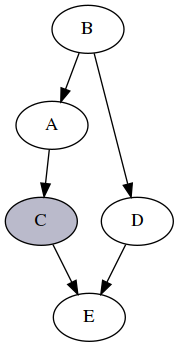
\includegraphics[width=0.5\linewidth]{images/Chapter 2/z-effect(1)}
%		\subcaption{$S=\emptyset$}
%		\label{fig:z-effect(a)}
%	\end{subfigure}
%	\begin{subfigure}{0.49\linewidth}
%		\centering
%		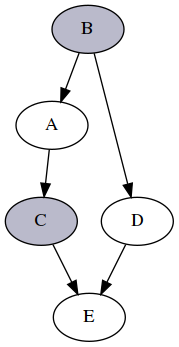
\includegraphics[width=0.5\linewidth]{images/Chapter 2/z-effect(2)}
%		\subcaption{$S = \{B\}$}
%		\label{fig:z-effect(b)}
%	\end{subfigure}
%	\caption{Identificación del efecto Z-específico}
%	\label{fig:z-effect}
%\end{figure}
%
%\subsection{El criterio de la puerta principal}
%El criterio de la puerta trasera no cubre todos los escenarios donde es posible aplicar el operador $do$. Existe otro criterio que nos puede ayudar en tales casos \cite{pearl2016causal}.
%\begin{dfn}[Criterio de la puerta principal]
%	Un conjunto de variables $\textbf{Z}$ se dice que satisface el criterio de la puerta principal relativo a un par ordenado de variables $(X,Y)$ si:
%	\begin{enumerate}
%		\item $\textbf{Z}$ intercepta todos los caminos dirigidos de $X$ hacia $Y$.
%		\item No hay ningún camino de puerta trasera de $X$ hacia $\textbf{Z}$ que esté desbloqueado.
%		\item Todos los caminos de puerta trasera de $\textbf{Z}$ hacia $Y$ son bloqueados por $X$.
%	\end{enumerate}
%\end{dfn}
%
%\begin{theorem}
%	Si $\textbf{Z}$ satisface el criterio de la puerta principal relativo a $(X,Y)$ y si $P(X,\textbf{Z}) > 0$, entonces el efecto causal de $X$ en $Y$ está dado por la fórmula:
%	\[P(Y=y|do(X=x)) = \sum_{\textbf{z}} P(\textbf{Z}=\textbf{z}|X=x) \sum_{x'} P(Y=y|X=x',\textbf{Z}=\textbf{z})P(X=x')\]
%\end{theorem}
%
%En el diagrama de la figura \ref{fig:frontdoor-ex} se puede comprobar que $\{Z\}$ satisface el criterio de la puerta principal relativo a $(X,Y)$ porque:
%\begin{enumerate}
%	\item Z intercepta el único camino dirigido de $X$ hacia $Y$: $X \rightarrow Z \rightarrow Y$.
%	\item El camino $X \leftarrow U \rightarrow Y \leftarrow Z$ está bloqueado por $U$.
%	\item El camino de puerta trasera $Z \leftarrow X \leftarrow U \rightarrow Y$ es bloqueado por $X$.
%\end{enumerate}
%\begin{figure}[!h]
%	\centering
%	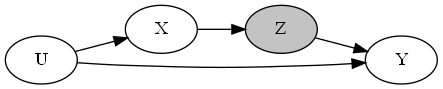
\includegraphics[width=0.50\linewidth]{images/Chapter 2/frontdoor.png.png}
%	\caption{Aplicación del criterio de la puerta principal}
%	\label{fig:frontdoor-ex}
%\end{figure}		
%
%\subsection{El cálculo-do}		
%El cálculo-do \cite{PearlMackenzie18} es un conjunto de reglas que nos permite transformar una expresión en otra con el objetivo de obtener una expresión final libre del operador $do$ que nos permita conocer el resultado de una intervención a partir de probabilidades preintervención:
%\begin{enumerate}
%	\item[\textbf{Regla 1:}] \[ P(Y|do(X), Z, W) = P(Y|do(X), Z) \] en el caso de que $Z$ bloquee todos los caminos de $W$ a $Y$ en el submodelo $M_x$.
%	
%	\item[\textbf{Regla 2:}] \[ P(Y|do(X), Z) = P(Y|X, Z) \] si $Z$ satisface el criterio de la puerta trasera.
%	
%	\item[\textbf{Regla 3:}] \[ P(Y|do(X)) = P(Y) \] si no existe un camino de $X$ hacia $Y$ con solo aristas hacia delante.		
%\end{enumerate}
%
%La Regla 1 nos dice que cuando observamos una variable $W$ luego de la intervención de $X$ y esta sea irrelevante a $Y$  condicionado a una variable $Z$, la distribución de probabilidad de $Y$ no cambiará. Por otro lado, la Regla 2 nos dice que una vez que ajustemos para cada variable de confusión, toda correlación que permanezca es un efecto causal genuino.	Por último, Regla 3 nos dice que si intervenimos una variable que no afecta a $Y$, entonces su distribución de probabilidad no se ve afectada.
%
%Cada regla tiene a su vez un significado sintáctico. La Regla 1 permite añadir o eliminar observaciones. La Regla 2 permite reemplazar una intervención por una observación y viceversa. La Regla 3 permite la adición o eliminación de intervenciones. 
%
%\subsection{Intervenciones mediante inferencia bayesiana}\label{sec:do-bn}
%Otra alternativa para calcular el efecto de una intervención es manipular el modelo $M$, obteniendo un submodelo $M_x$ en el que calcular el efecto de la intervención $P(Y=y \mid do(X=x))$ se reduce a convertir la variable intervenida en una observación y calcular $P_m(Y=y \mid X=x)$. Una vez obtenido este modelo, se puede construir una red bayesiana a partir del mismo mediante el procedimiento descrito en la sección \ref{secc:scm-bn}. Posteriormente se instancian las variables observadas y se aplica un algoritmo de inferencia bayesiana para obtener la respuesta a la consulta deseada.
%
%\section{Contrafactuales}		
%Los contrafactuales son utilizados para comparar dos posibles salidas de una variable, exactamente bajo las mismas condiciones, excepto en una que difiere. Por ejemplo, para aliviar un malestar un individuo decide tomar un medicamento, recuperándose en 6 horas. Este podría preguntarse: Dado que tomé el medicamento y me recuperé en 6 horas, \textquestiondown cuál sería el tiempo de recuperación si no lo hubiese tomado ? Para responder a la pregunta, existen tres variables que deben ser tenidas en cuenta:
%\begin{itemize}
%	\item $Y_{x=1}$ es el tiempo de recuperación si se toma el medicamento.
%	\item $Y_{x=0}$ es el tiempo de recuperación si no se toma.
%	\item $X$ representa la decisión de tomar o no el medicamento.	
%\end{itemize}
%Luego, la expresión que responde a la pregunta es:
%\[ E(Y_{x=0}|X=1,Y_{x=1}=6) \]
%Note que $Y_{x=1}$ y $Y_{x=0}$ corresponden a la misma variable pero con un antecedente distinto. La expresión anterior es distinta de $E[Y \mid do(X=0), Y=6]$ porque esta última no tiene en cuenta la diferencia entre el tiempo de recuperación dado que se tomó medicamento del tiempo de recuperación dado que no se tomó. Esta diferencia plantea la existencia de dos mundos: el mundo real, donde el individuo toma el medicamento y se recupera en 6 horas, y un mundo alternativo, donde el individuo no toma el medicamento y podría, por tanto, experimentar un tiempo de recuperación distinto al del mundo real.
%
%\subsection{Contrafactuales deterministas}		
%Sea $M$ un SCM completamente especificado, donde se conocen tanto las funciones ($F$) como los valores de todas las variables exógenas. En dicho modelo cada asignación $\textbf{U}=\textbf{u}$ a las variables exógenas identifica a un individuo de la población
%o situación particular en la naturaleza del problema. Consideremos la sentencia contrafactual: \textquotedblleft $Y$ hubiese tomado el valor $y$, si $X$ hubiese tomado el valor $x$, en la situación $\textbf{U}=\textbf{u}$\textquotedblright, denotada como $Y_x(\textbf{u})=y$ donde $Y$ y $X$ son dos variables en $V$. Este tipo de contrafactual se denomina \textit{determinista}, porque corresponde a un individuo de la población del que conocemos el valor de cada variable relevante. Supongamos que se tiene información de un individuo mediante la evidencia $\textbf{E}=\textbf{e}$, que asigna a cada variable endógena un valor.  Para calcular el contrafactual determinista $Y_x(\textbf{u})=y$ en base a la evidencia $\textbf{e}$ se debe seguir el siguiente algoritmo \cite{pearl2016causal}:
%
%\begin{enumerate}
%	\item Abducción: Usar la evidencia $\textbf{E}=\textbf{e}$  para determinar el valor de $\textbf{U}$. Este paso explica el pasado, ($\textbf{u}$) en base a la evidencia actual $\textbf{e}$.
%	\item Acción: Modificar el modelo $M$, reemplazando las ecuaciones que definen a $X$ por la función apropiada $X=x$, para obtener un modelo modificado $M_x$. Este paso cambia el curso de la historia (mínimamente) para cumplir con la hipótesis del contrafactual.
%	\item Predicción: Usar $M_x$ y el valor de $\textbf{U}$ para computar el valor de $Y$, la consecuencia del contrafactual. Este paso predice el futuro ($Y$) basado en el nuevo entendimiento del pasado y la nueva condición establecida.
%\end{enumerate}
%
%Ilustremos este procedimiento mediante un ejemplo. Un conductor debe moverse desde su hogar a su trabajo. Durante el recorrido, se encuentra con un desvío que igual conduce a su destino pero no decide tomarlo. Una vez llegado a su centro de trabajo, nota que le tomó media hora el recorrido habiéndose movido a una velocidad media de $50$ km/h y se pregunta cuánto se hubiese demorado yendo a la misma velocidad pero tomando el desvío. Un modelo causal para esta situación podría ser el siguiente:		
%\begin{align*}
%	&D=U_d\\
%	&V=U_v\\
%	&T=	\frac{25 - 5 \cdot D}{V} + U_t
%\end{align*}
%En este caso $D$ es una variable binaria que representa la decisión de tomar el desvío y toma valor $1$ en caso afirmativo y $0$ en caso contrario, $V$ la velocidad a la que se mueve el conductor (en km/h) y $T$ el tiempo que este demora en llegar a su destino (en horas). Siguiendo los pasos listados en el algoritmo anterior:
%
%\begin{enumerate}
%	\item Abducción:
%	Primeramente obtenemos los valores de $U_d$, $U_v$ y $U_t$ a partir de la evidencia, sustituyendo los valores $D=0$, $V=50$ y $T=0.5$ en las ecuaciones del modelo y despejando las variables deseadas.
%	\begin{align*}
%		&U_d = D = 0\\
%		&U_v = V = 50\\
%		&U_t = T -  \frac{25 - 5 \cdot D}{V} = 0.5 - \frac{25 -5(0)}{50} = 0			
%	\end{align*}
%	\item Acción:
%	Luego corresponde modificar el modelo, sustituyendo la ecuación que define a $D$ por $D=1$:
%	\begin{align*}
%		&D = 1\\
%		&V = U_v\\
%		&T = \frac{25 - 5 \cdot D}{V} + U_t		
%	\end{align*}				
%	\item Predicción:
%	Por último, predecimos la variable deseada, haciendo uso de los valores de $\textbf{U}$ y del modelo $M_d$ computados anteriormente.
%	\begin{align*}
%		&T_{D=1}(U_d=1, U_v=50, U_t=0)\\
%		&=\frac{25 - 5 \cdot 1}{50} + 0\\
%		&=0.4			
%	\end{align*}	
%\end{enumerate}
%
%Por tanto, tomar el desvío le hubiese hecho llegar antes al trabajo.
%
%\subsection{Contrafactuales no deterministas}			
%Los contrafactuales pueden utilizarse también en el caso no determinista para estudiar el comportamiento de las variables en una clase o rango de la población. La expresión $P(Y_x=y \mid \textbf{E}=\textbf{e})$ expresa la probabilidad de que la variable $Y$ tomase el valor $y$ si se fijara el valor de $X$ a $x$ en individuos donde se observa la evidencia $\textbf{E}=\textbf{e}$.
%
%El procedimiento para calcular contrafactuales deterministas puede modificarse para el caso no determinista como se muestra a continuación \cite{pearl2016causal}:
%
%\begin{enumerate}
%	\item Abducción: Actualizar $P(\textbf{U})$ a partir de la evidencia $\textbf{E}=\textbf{e}$ para obtener $P(\textbf{U} \mid \textbf{E}=\textbf{e})$.
%	
%	\item Acción: Modificar el modelo $M$, reemplazando las ecuaciones que definen a las variables en $X$ por la apropiada asignación $X=x$ para obtener el modelo modificado $M_x$.
%	
%	\item Predicción: Usar el modelo modificado $M_x$, y las probabilidades actualizadas sobre las variables de $\textbf{U}$, $P(\textbf{U} \mid \textbf{E}=\textbf{e})$, para calcular la probabilidad de $Y_x$, la respuesta al contrafactual.
%\end{enumerate}
%
%\subsection{Contrafactuales mediante inferencia bayesiana}
%Al igual que en las intervenciones, la inferencia bayesiana puede utilizarse en la resolución de contrafactuales, una vez que estos sean definidos en términos de datos recogidos de observaciones. A partir del procedimiento para computar contrafactuales no deterministas mostrado en la sección anterior, es posible diseñar un algoritmo que calcule contrafactuales utilizando la inferencia bayesiana. Los pasos a seguir por el algoritmo se describen a continuación:
%
%\begin{enumerate}
%	\item Construir una red bayesiana $N$ a partir del modelo $M$.
%	\item Realizar inferencia en la red para obtener las creencias actualizadas de las variables exógenas a partir de la introducción de la evidencia $E=e$(abducción).
%	\item Modificar la red de tal forma que se refleje la transformación del modelo original $M$ en el submodelo $M_x$, eliminando todas las aristas que inciden en el nodo de la variable $X$ pero preservando las probabilidades que se actualizaron en el paso anterior(acción)
%	\item Instanciar tanto la variable intervenida $X$ como las variables observadas observaciones y aplicar inferencia en la red para obtener la respuesta al contrafactual(predicción).				
%\end{enumerate}
%
%Este método ofrece una alternativa intuitiva para calcular contrafactuales. Su inconveniente es la gran cantidad de recursos que demanda al tener que realizarse dos veces un algoritmo de inferencia cuya complejidad es exponencial.		
%
%\subsection{Método de las redes gemelas}\label{sec:tn}
%El método de las redes gemelas \cite{grahamcopy, balke1995probabilistic} ofrece una alternativa al algoritmo anterior para reducir el costo computacional. Este se basa igualmente en la inferencia bayesiana. Para ello se expande el modelo original $M$, construyendo un nuevo modelo $M'$ cuyo grafo causal consiste en dos redes idénticas en estructura interconectadas. Una representa el mundo real y otro el alternativo. Formalmente $M'=\langle U',V',F'\rangle$ donde:
%\begin{itemize}
%	\item $U'= U$. El conjunto de las variables exógenas se mantiene intacto.
%	\item $V' = V \cup V^{\ast}$ donde $V^{\ast}=\{V_i^{\ast}: V_i \in V \}$. Se crea una variable endógena idéntica a cada variable del modelo original, pero etiquetada con un nombre distinto. Las variables de $V^{\ast}$ corresponden al mundo alternativo.
%	\item $F' = F \cup F^{\ast}$ donde $F^{\ast}=\{F_{V_i}^{\ast}: F_{V_i} \in F\}$. Cada variable $V_i^{\ast}$ poseerá una función $F_{V_i}^{\ast}$ que resultará semejante a la de su gemela pero cuyos argumentos corresponderán a las variables del mundo alternativo.
%\end{itemize}
%
%Una vez construidas las redes gemelas se representa en el mismo modelo tanto el mundo real como el mundo alternativo. Supongamos que se quiere calcular el contrafactual $P(Y_x=y \mid Z=z)$. En el modelo de las redes gemelas $M'$ se cumple que:
%
%\[P(Y_x=y \mid Z=z) = P'(Y^{\ast}=y \mid do(X^{\ast}=x), Z=z)\]
%De esta forma, calcular un contrafactual en el modelo original se reduce a calcular una intervención en el modelo de las redes gemelas. Podemos ir más allá y utilizando el algoritmo visto en la sección de intervención en redes bayesianas, obtener un modelo $M'_x$ que simule la intervención de $X$ y donde se cumpla que:
%
%\[P'(Y^{\ast}=y \mid do(X^{\ast}=x), Z=z) = P'_m(Y^{\ast}=y \mid X^{\ast}=x, Z=z)\].
%Por tanto calcular un contrafactual en el modelo original $M$ puede reducirse a predecir el valor de una variable a partir de observaciones en el modelo resultante de intervenir el modelo de las redes gemelas $M'_x$. Para calcular esta predicción puede transformarse el modelo en una red bayesiana y aplicar un algoritmo de inferencia.
%
%Para disminuir el costo computacional de la inferencia en una red de tamaño igual al doble de la original se puede utilizar el método de mezcla de nodos \cite{shpitser2012counterfactuals}. Por cada nodo $X^{\ast}$ del mundo alternativo, si este no desciende de un nodo intervenido ni de un nodo que corresponde a una de las variables que queremos estimar, se puede mezclar con su correspondiente nodo del mundo real $X$, conformando un único nodo $X'$ donde $Pa_X' = Pa_X \cup Pa_X^{\ast}$ y $Ch_X' = Ch_X \cup Ch_X^{\ast}$. Este nodo toma los mismos valores que $X$ y $X^{\ast}$ y la misma función de definición que $X$. 
%
%En resumen, calcular un contrafactual en un SCM puede resumirse en el siguiente algoritmo:
%
%\begin{enumerate}
%	\item Construir el modelo de redes gemelas $M'$ a partir de $M$.
%	\item Obtener el modelo $M'_x$ a partir de $M'$, resultante de la intervención $X=x$.
%	\item Reducir el tamaño del modelo $M'_x$ mediante la mezcla de nodos, obteniendo un modelo $M''_x$
%	\item Construir una red bayesiana $N$ a partir de $M''_x$.
%	\item Calcular $P'_m(Y*=y \mid X^{\ast}=x, Z=z)$ en $N$, aplicando un algoritmo de evidencia bayesiana.
%\end{enumerate}
%
%La figura \ref{fig:count-tn} muestra el proceso de transformaciones que va sufriendo la red a lo largo de la ejecución del algoritmo para calcular el contrafactual $P(W_z=w\mid Y=y)$. La figura \ref{fig:count-tn-a} muestra el modelo original, \ref{fig:count-tn-b} el modelo de las redes gemelas, \ref{fig:count-tn-c} el submodelo resultante de intervenir las redes gemelas, \ref{fig:count-tn-d} el modelo resultante de aplicar mezcla de nodos al submodelo y \ref{fig:count-tn-e} la red bayesiana construida y con las correspondientes variables instanciadas. 
%
%\begin{figure}
%	\centering			
%	\begin{subfigure}{0.49\linewidth}
%		\centering
%		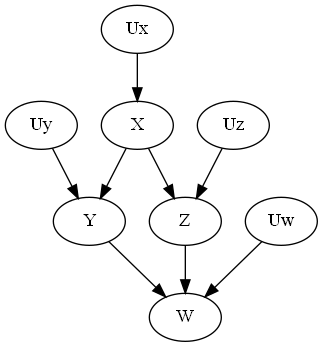
\includegraphics[width=0.7\linewidth]{./images/Chapter 2/count-tn-1.png}
%		\caption{}
%		\label{fig:count-tn-a}
%	\end{subfigure}
%	\begin{subfigure}{0.49\linewidth}
%		\centering
%		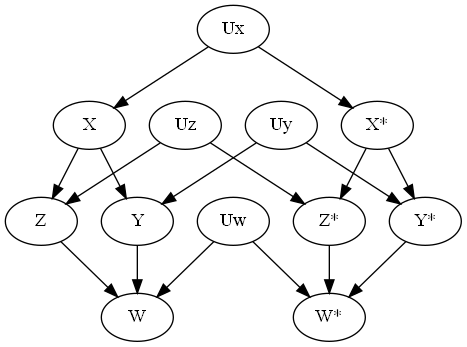
\includegraphics[width=\linewidth]{./images/Chapter 2/count-tn-2.png}
%		\caption{}
%		\label{fig:count-tn-b}
%	\end{subfigure}
%	\begin{subfigure}{0.49\linewidth}
%		\centering
%		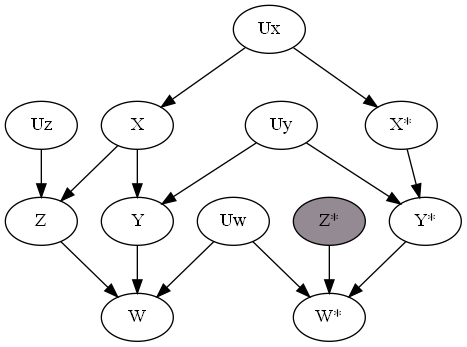
\includegraphics[width=\linewidth]{./images/Chapter 2/count-tn-3.png}
%		\caption{}		
%		\label{fig:count-tn-c}
%	\end{subfigure}
%	\begin{subfigure}{0.49\linewidth}
%		\centering
%		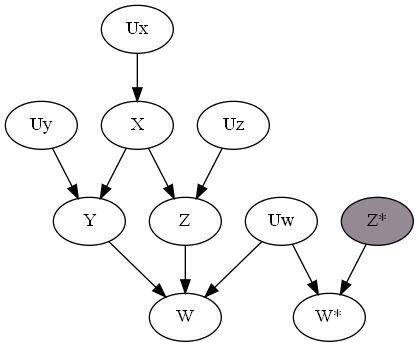
\includegraphics[width=\linewidth]{./images/Chapter 2/count-tn-4.png}
%		\caption{}
%		\label{fig:count-tn-d}
%	\end{subfigure}
%	\begin{subfigure}{0.49\linewidth}
%		\centering
%		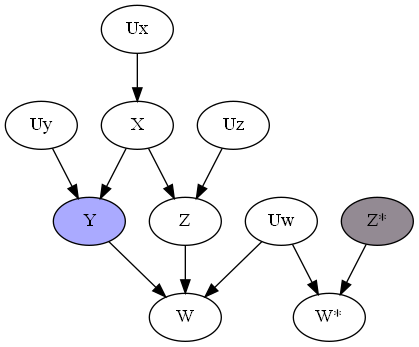
\includegraphics[width=\linewidth]{./images/Chapter 2/count-tn-5.png}
%		\caption{}
%		\label{fig:count-tn-e}
%	\end{subfigure}			
%	\caption{Aplicación del método de las redes gemelas para calcular un contrafactual}
%	\label{fig:count-tn}
%\end{figure}
%
%\section{Atribución} \label{sec:attr}
%Consideremos el ejemplo de una persona que contrae una enfermedad y para eliminarla decide tomar un medicamento. Un tiempo después, dicha persona se recupera y se hace la pregunta: \textquestiondown Realmente fue tomar el medicamento lo que me hizo recuperarme de la enfermedad ?. La probabilidad de necesidad (PN) mide el grado en que tomar el medicamento $X=1$ es necesario para recuperarse de la enfermedad($Y=1$). El valor de $PN$ lo determina la probabilidad de que no exista recuperación si no se toma el medicamento, dado que se tomó el medicamento y hubo recuperación:
%\[PN=P(Y_0=0|Y=1,X=1)\]
%
%Por otro lado, puede darse el caso de un individuo que no tome el medicamento y no se recupere de la enfermedad. En tal caso, dicho individuo podría hacerse la pregunta: \textquestiondown Si hubiese tomado el medicamento me hubiese recuperado ?  La probabilidad de suficiencia (PS) indica el grado en que la acción no realizada (tomar el medicamento) hubiese sido suficiente para lograr el efecto contrario, es decir, recuperarse ($Y=1$). Matemáticamente, es equivalente a la probabilidad de que el individuo se hubiese recuperado si hubiese tomado el medicamento, dado que no lo tomó y no hubo recuperación.
%\[PS = P(Y_1=1|X=0,Y=0)\]
%
%Imaginemos un tercer individuo que padece la enfermedad. \textquestiondown Y si resulta que la enfermedad está en una fase terminal, y tomar o no el medicamento no influirá en la recuperación del mismo? \textquestiondown Y si en realidad no necesita tomar el medicamento puesto que su sistema inmunológico por si solo puede combatir la enfermedad ? La única razón para que dicho individuo tome el medicamento es que haciéndolo se recuperará y si no lo toma entonces no se recuperará. En otras palabras, lo que quiere determinar el individuo es la probabilidad de que tomar el medicamento sea una condición necesaria y suficiente para su recuperación:
%\[ PNS = P(Y_1=1, Y_0=0) \]		
%
%Las tres probabilidades anteriores, $PN$, $PS$ y $PNS$ son ejemplos del uso de la causalidad para atribuir un efecto (recuperarse) a una causa (tomar un medicamento). A continuación se definen formalmente \cite{pearl2016causal}:
%
%\begin{dfn}
%	Sean $X$ y $Y$ variables binarias en un modelo causal $M$. Sean $x$, $y$ los valores que corresponden a las asignaciones X=verdadero y Y=verdadero respectivamente. A su vez, sean $x'$, $y'$ los valores de sus respectivos complementos. Se definen las siguientes probabilidades:			
%	\begin{itemize}
%		\item \textbf{Probabilidad de necesidad (PN):}
%		\[PN=P(Y_{x'}=y'|Y=y,X=x)\]
%		\item \textbf{Probabilidad de suficiencia (PS):}
%		\[PS = P(Y_x=y|X=x',Y=y')\]
%		\item \textbf{Probabilidad de necesidad y suficiencia (PNS):}
%		\[ PNS = P(Y_x=y, Y_{x'}=y') \]
%	\end{itemize}			
%\end{dfn}
%
%En el caso de la $PNS$, resulta imposible calcularla experimentalmente a partir de la definición provista. Sin embargo, es posible definirla en términos de $PN$ y $PS$ \cite{pearl_2009}: 
%
%\begin{prop}
%	Las probabilidades $PN$, $PS$ y $PNS$ satisfacen la siguiente relación :
%	\[ PNS = P(x,y)PN + P(x',y')PS \]
%\end{prop}
%
%\section{Mediación}\label{sec:med}
%El modelo canónico para un problema de mediación toma la siguiente forma:
%\[
%\arraycolsep=10pt
%\begin{array}{ccc}
%	x = f_X(U_X)&
%	m = f_M(x, u_M)&
%	y = f_Y(x, m , u_Y)
%\end{array}
%\]
%donde $X$(origen), $M$(mediador) y $Y$(destino) son variables aleatorias, $f_X$, $f_M$ y $f_Y$ son funciones y $U_X$, $U_M$ y $U_Y$ son los factores omitidos que actúan sobre las variables $X$, $M$ y $Y$ respectivamente (Figura \ref{fig:mediation}). Se asume además que los factores omitidos son independientes entre sí.
%
%\begin{figure}[!h]
%	\centering
%	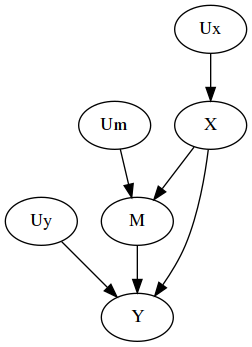
\includegraphics[width=0.35\linewidth]{./images/Chapter 2/mediation.png}
%	\caption{Modelo canónico para análisis de mediación}
%	\label{fig:mediation}
%\end{figure} 
%
%Teniendo el cuenta el modelo anterior, existen cuatro tipos de efectos diferentes que describen la transición de $X=x$ hacia $X=x'$ \cite{pearl2016causal}. Sin perder generalidad, supongamos que $x=0$ y $x'=1$.
%
%\begin{enumerate}
%	\item \textbf{Efecto total}
%	\begin{align*}
%		TE &= E[Y_1 - Y_0]\\
%		&=E[Y \mid do(X=1)] - E[Y \mid do(X=0)]
%	\end{align*}
%	El efecto total mide el incremento esperado en $Y$ cuando $X$ cambia de $X=0$ hacia $X=1$, mientras que $M$ toma su valor natural, dictado por la función $f_M$
%	
%	\item \textbf{Efecto directo controlado}
%	\begin{align*}
%		CDE(m)
%		&=E[Y_{1,m} - Y_{0,m}] \\
%		&=E[Y \mid do(X=1,M=m)] - E[Y \mid do(X=0,M=m)]
%	\end{align*}
%	
%	El efecto directo controlado mide el incremento esperado en $Y$ cuando $X$ cambia de $X=0$ hacia $X=1$ y el mediador $M$ es forzado a tomar un valor $m$.
%	
%	\item \textbf{Efecto directo natural}
%	\begin{align*}
%		NDE
%		&=E[Y_{1,M_0} - Y_{0,M_0}] \\
%		&=E[Y \mid do(X=1,M=M_0)] - E[Y \mid do(X=0,M=M_0)]
%	\end{align*}
%	
%	El efecto directo natural mide el incremento esperado en $Y$ cuando $X$ cambia de $X=0$ a $X=1$ y el mediador $M$ obtiene el valor que hubiese tomado en caso de que $X$ fuese forzado a tomar el valor $X=0$.
%	
%	\item \textbf{Efecto indirecto natural}
%	\begin{align*}
%		NIE
%		&=E[Y_{0,M_1} - Y_{0,M_0}] \\
%		&=E[Y \mid do(X=0,M=M_1)] - E[Y \mid do(X=0,M=M_0)]
%	\end{align*}
%	
%	El efecto indirecto natural mide el incremento esperado en $Y$ cuando $X$ se mantiene con el valor fijo $X=0$ y el mediador cambia de $M_0$ a $M_1$.
%\end{enumerate}
%
%Supongamos que se quiere determinar si existe discriminación por género en las entrevistas de contratación para un trabajo. Se dispone de un modelo como el de la figura \ref{fig:mediation} que representa la relación entre el género del entrevistado ($X$), su calificación en la entrevista ($M$) y si este es contratado ($Y$). Para determinar si existe discriminación se puede utilizar el efecto directo controlado, asignándoles un valor de calificación fijo $m$ a la población de estudio y utilizando la fórmula vista para el CDE, donde $X=1$ representa el sexo femenino y $X=0$ el masculino y por otro lado $Y=1$ indica que el entrevistado fue contratado y $Y=0$ indica el caso contrario. Si se obtiene un valor negativo, ello indica que las mujeres son más propensas a no ser aceptadas en una entrevista de trabajo por discriminación.

	\chapter{Propuesta de software}

Se desarrolló un programa capaz de brindar al usuario la posibilidad de realizar operaciones de inferencia causal. Las características que reúne el programa son las siguientes:
\begin{enumerate}
	\item Ofrecer una interfaz visual que permita a usuarios no expertos en programación realizar operaciones de inferencia causal. Dicha interfaz debe asistir al usuario tanto en la creación de los modelos como en las operaciones de inferencia causal, notificándolo en el caso de que existan errores en la entrada provista. 
	\item Permitir la construcción y visualización de SCMs. Debe permitir además exportar los modelos a ficheros externos para posteriormente ser cargados en el programa.
	\item Permitir realizar operaciones de inferencia causal sobre modelos causales estructurales. Ofrecer en un menú los distintos tipos de inferencia causal disponibles. Permitir al usuario seleccionar los parámetros que el programa tendrá en cuenta durante la inferencia.
	\item Ofrecer los resultados correspondientes a la consulta causal especificada por el usuario.
\end{enumerate}

\section{Implementación}		
El lenguaje de programación escogido para la implementación fue \textbf{Python} en su versión $3.8$. Su elección se debe a que es un lenguaje de alto nivel, multiparadigma  y con una filosofía que apuesta por un código legible y sencillo.

La implementación de la parte lógica del proyecto consiste de 3 módulos contenidos en un directorio llamado \textit{causality}. Estos módulos son:
\begin{itemize}
	\item \textit{main.py}: Contiene la implementación del SCM.
	\item \textit{tests.py}: Conjunto de tests unitarios destinados a probar las componentes fundamentales de la implementación.
	\item \text{util.py}: Conjunto de métodos auxiliares que serán utilizados desde otros módulos.
\end{itemize}

\subsection{Implementación del modelo causal estructural}
En el módulo \textit{main.py} se trabaja con un conjunto de clases para la implementación del modelo:	  

\begin{lstlisting}
	class Variable:
		def __init__(self, name, values):...
	
	class ExogenousVariable(Variable):
		def __init__(self, name, values, distribution):...
	
	class EndogenousVariable(Variable):
		def __init__(self, name, values, parents, expression):...
	
	class SCM:
		def __init__(self, exogenous_variables, endogenous_variables):...
\end{lstlisting}

La clase \textit{Variable} reúne las características comunes de las variables tanto exógenas como endógenas. Debe proveerse un nombre para la variable que la identifique en el modelo, por lo que este debe ser único. Además debe proveerse una lista de los valores que la variable puede tomar. La naturaleza de las variables es discreta y estas solo pueden tomar valores numéricos. Esta clase no se utiliza directamente sino que es heredada por las clases \textit{ExognousVariable} y \textit{EndogenousVariable}. 

La clase \textit{ExogenousVariable} representa a las variables exógenas de un SCM. Para crear una variable exógena se debe especificar su nombre, los valores que toma y su distribución de probabilidad. Dicha distribución consiste en una lista $P$ donde cada valor $P[i]$ se corresponde con la probabilidad de que la variable tome el valor $V[i]$, donde $V$ es la lista de valores provista. La lista debe cumplir con todas las propiedades de una distribución de probabilidad:
\begin{itemize}
	\item La suma de sus valores debe ser igual a 1
	\item Cada valor debe ser encontrarse en el intervalo $[0,1]$
\end{itemize}

En el caso de las variables endógenas, representadas por la clase \textit{EndogenousVariable} debe especificarse el nombre, los valores que toma, los padres de la variable (variables de las que depende) y la expresión que define a la misma. Es importante especificar todos los posibles valores que puede tomar la variable a partir de las variables de las que depende. Toda variable endógena debe depender de al menos otra variable y una de estas variables debe ser exógena. Esto último es necesario para el cálculo correcto de los contrafactuales, ya que el método utilizado (redes gemelas) utiliza las variables exógenas para conectar las variables del mundo real con las del mundo alternativo.

La expresión que define a la variable será una cadena con una sintaxis similar a las expresiones de Python. Además se podrán usar funciones de la clase \textit{math}, que viene integrada a dicho lenguaje. Ejemplo de posibles expresiones válidas son:
\begin{itemize}
	\item X + Y - 1
	\item (X and Y) if Z == 0 else (X or Y)
	\item max(X, Y) - min(X,Y)
\end{itemize}
Las variables que aparecen en las expresiones deben corresponderse con los nombres de las variables de las que depende la variable que se está definiendo.

Una vez creadas las variables exógenas y endógenas, estas se agrupan en dos listas y se llama al constructor de la clase $SCM$, la cual representa a los modelos causales estructurales.

Por ejemplo, si se tiene un modelo como el siguiente:

\begin{model}
	\label{model:sum}
	\[
	\arraycolsep=10pt
	\begin{array}{ccc}
		U = \{Ux, Uy, Uz\}&
		V = \{X, Y, Z\}&
		E = \{f_x, f_y, f_z\}
	\end{array}
	\]
	
	\[Val(Ux)=Val(Uy)=Val(X)=Val(Y)=\{0,1,2\}\]
	\[Val(Uz)=\{0, 1\}\]
	\[Val(Z)=\{0, 1, 2, 3, 4\}\]
	
	\begin{equation*}
		P(X=x)=  
		\left\{
		\begin{array}{ll}
			0.1 & \mathrm{si\ } x = 0\\
			0.2 & \mathrm{si\ } x = 1\\
			0.7 & \mathrm{si\ } x = 2\\
		\end{array}
		\right\}.
	\end{equation*}
	
	\begin{equation*}
		P(Y=y)=  
		\left\{
		\begin{array}{ll}
			0.2 & \mathrm{si\ } y = 0\\
			0.2 & \mathrm{si\ } y = 1\\
			0.6 & \mathrm{si\ } y = 2\\
		\end{array}
		\right\}.
	\end{equation*}
	
	\begin{equation*}
		P(Z=z)=  
		\left\{
		\begin{array}{ll}
			0.8 & \mathrm{si\ } z = 0\\
			0.2 & \mathrm{si\ } z = 1\\
		\end{array}
		\right\}.
	\end{equation*}
	
	\begin{center}
		\[
		\begin{array}{cc}
			f_x: & X = Ux\\
			f_y: & Y = Uy\\	
		\end{array}
		\]			
		\begin{equation*}
			f_z: Z=  
			\left\{
			\begin{array}{ll}
				X + Y & \mathrm{si\ } Uz = 0\\
				X * Y & \mathrm{si\ } Uz = 1\\
			\end{array}
			\right\}.
		\end{equation*}
	\end{center}
\end{model}

Entonces para construir dicho modelo se usaría el código:

\begin{lstlisting}
	Ux = ExogenousVariable("Ux", [0, 1, 2], [0.1, 0.2, 0.7])
	Uy = ExogenousVariable("Uy", [0, 1, 2], [0.2, 0.2, 0.6])
	Uz = ExogenousVariable("Uz", [0, 1], [0.8, 0.2])
	
	X = EndogenousVariable("X", [0, 1, 2], [Ux], "X")
	Y = EndogenousVariable("Y", [0, 1, 2], [Uy], "Y")
	Z = EndogenousVariable("Z", [0, 1, 2, 3, 4], [X, Y, Uz], "X + Y if Uz == 0 else X * Y")
	
	model = SCM([Ux, Uy, Uz], [X, Y, Z])
\end{lstlisting}

Los modelos también tienen una representación en formato JSON (Javascript Object Notation) con el objetivo de persisitirlos en ficheros y así poder usarlos posteriormente. El método \textit{export\_to\_json} convierte un objeto de tipo SCM a su representación en JSON, mientras que el método \textit{import\_from\_json} crea un objeto de tipo SCM a partir de la representación en JSON correspondiente. A su vez, los métodos \textit{export\_to\_json\_file} e \textit{import\_from\_json\_file} permiten guardar y cargar de memoria externa respectivamente.

\subsection{Algoritmos de inferencia}
La implementación de los algoritmos de inferencia causal se basa en la inferencia bayesiana. A la hora de responder a una pregunta causal se aplica un algoritmo que en algún punto pasa por la construcción de una red bayesiana y la ejecución de un algoritmo de inferencia para obtener la respuesta deseada.

Para el trabajo con redes bayesianas se utilizó la librería \textbf{pgmpy} \cite{ankan2015pgmpy}. Esta es una librería de código abierto para el trabajo con redes bayesianas, enfocada en la modularidad y la extensibilidad. Contiene implementaciones de algoritmos de estimación de parámetros, aprendizaje de estructura, inferencia exacta, aproximada y además inferencia causal.

El método \textit{build\_bayesian\_network} construye una red bayesiana a partir de un modelo causal estructural, mediante un proceso similar al descrito en la sección \ref{secc:scm-bn}. La parte más compleja de dicho algoritmo consiste en la creación de las tablas de probabilidad de las variables endógenas, donde es necesario computar todas las combinaciones posibles de valores que pueden tomar los padres más la variable. Así, si una variable $X$ depende de un conjunto $Pa_X=\{P_1, P_2, ..., P_n\}$ de variables, su tabla de probabilidad contaría con $|X| \cdot \prod_{i=1}^n |P_i|$ entradas, donde $|P_i|$ denota la cardinalidad de la variable $P_i$ y $|X|$ la cardinalidad de $X$. Para determinar el valor de cada probabilidad $P(X_i=x_i \mid Pa_X=x^{\ast})$ se evalúa la expresión que define a $X$ en la correspondiente asignación $x^{\ast}$ a las variables padres de $X$. Si el resultado es igual a $x_i$, entonces la probabilidad toma valor 1. En caso contrario toma valor 0. Para evaluar la expresión se utiliza la función \textit{eval} integrada a Python, que toma una expresión en forma de cadena de caracteres y los valores que se le asigna a las variables, y devuelve el resultado de evaluar dicha expresión.

Existen 3 tipos principales de inferencia en la implementación: predicciones, intervenciones y contrafactuales. Las signaturas de los métodos correspondientes a dichas operaciones se definen a continuación:

\begin{lstlisting}
	def predict(self, variables, observations={}, map=False, joint=False, algorithm="BP"):...
	
	def do_bayesian(self, variables, do_variables, observations={}, map=False, joint=False, algorithm="BP"):...
	
	def counterfactual(self, variables, do_variables, observations={}, map=False, joint=False, algorithm="BP"):...
\end{lstlisting}

El método \textit{predict} permite realizar una predicción en el modelo, devolviendo las probabilidades actualizadas de un conjunto de variables solicitadas (parámetro \textit{variables}) a partir de un conjunto de variables observadas (\textit{observations}). Por ejemplo, si se quiere determinar la probabilidad $P(Y \mid X=1)$ se hece la llamada siguiente al método:	
\begin{lstlisting}
	result = model.predict(["Y"], observations={"X": 1})
\end{lstlisting}	
El método \textit{do\_bayesian} calcula el resultado de una intervención, incorporando el parámetro \textit{do\_variables} que indica las variables que son intervenidas y los valores que son forzados a tomar. Suponiendo que se quiere calcular $P(Y \mid do(X=1), Z=2)$ la llamada al método sería:
\begin{lstlisting}
	result = model.do_bayesian(["Y"], {"X": 1}, observations={"Z": 2})
\end{lstlisting}

Para calcular el resultado de la intervención se usa el procedimiento descrito en la sección \ref{sec:do-bn}: se construye el submodelo correspondiente a la intervención mediante el método \textit{get\_submodel}, y convirtiéndolo en red bayesiana con el método \textit{build\_bayesian\_network} se aplica inferencia para obtener la respuesta deseada. 

El método \textit{counterfactual} calcula el resultado de un contrafactual, recibiendo los mismos parámetros que el método \textit{do\_bayesian} pero con un significado ligeramente distinto: las variables de la respuesta deben corresponder al mundo alternativo, para lo cual se debe añadir el caracter \textquoteleft*\textquoteright al final del nombre de la variable, y lo mismo ocurre con las variables especificadas en \textit{do\_variables} que corresponden a las intervenciones realizadas en el mundo alternativo. Para calcular el contrafactual $P(Y_{X=1} \mid Z=z)$ la llamada al método \textit{counterfactual} sería:
\begin{lstlisting}
	result = model.counterfactual(["Y*"], {"X*": 1},observations={"Z": 2})
\end{lstlisting}
Para calcular el contrafactual se utiliza el método de las redes gemelas descrito en la sección \ref{sec:tn}. Se construye la estructura mediante el método \textit{build\_twin\_network} que a partir de un modelo construye el modelo de redes gemelas correspondiente. La respuesta al contrafactual se obtiene llamando al método \textit{do\_bayesian} sobre el modelo de redes gemelas resultante.

Los métodos anteriores disponen de un conjunto de parámetros opcionales . El parámetro \textit{map} especifica si en vez de realizar inferencia probabiliística se debe realizar inferencia MAP. El parámetro \textit{joint} indica si se desea obtener en la respuesta la distribución de probabilidad conjunta o las distribuciones por separado. El parámetro \textit{algorithm} indica el algoritmo de inferencia que será usado y puede tomar dos valores: \textquotedblleft BP \textquotedblright(propagación de creencias) y \textquotedblleft VE\textquotedblright(eliminación de variables).	

En caso de que la inferencia especificada sea probabilística, los métodos \textit{predict}, \textit{do\_bayesian} y \textit{counterfactual} devuelven una función. Si es solicitada la distribución conjunta, esta recibe como parámetro una asignación en forma de diccionario de los valores que toma cada variable y devuelve la probabilidad correspondiente. Si no se pide la distribución conjunta, entonces la función devuelta recibe como parámetro el nombre de una variable de la respuesta y el valor que toma, devolviendo la probabilidad correspondiente. Por otro lado, si se especifica que la inferencia es de tipo MAP, entonces se devuelve un diccionario con la asignación más probable a las variables.

Por ejemplo, para el modelo \ref{model:sum}, si deseamos obtener el valor de $P(Z_{X=1}=3 | Z=3)$, la instrucción de código quedaría:
\begin{lstlisting}
	model.counterfactual(["Z*"], {"X*": 1}, {"Z": 3})("Z*", 3)
\end{lstlisting}
En cambio la probabilidad conjunta $P(Z=3, Y=2 | do(X=1))$ se obtendría así:
\begin{lstlisting}
	model.do_bayesian(["Z", "Y"], {"X": 1})({"Z": 3, "Y": 2})
\end{lstlisting}
Por otro lado la asignación más probable MAP($Z, Y | do(X=1)$) se obtendría leyendo el diccionario que devuelve el llamado al método \textit{do\_bayesian\_map}:
\begin{lstlisting}
	result = model.do_bayesian(["Y", "Z"], {"X": 1}, map=True)
	for variable, value in result.items():
		print(variable, value)
\end{lstlisting}

Como se vio en las secciones \ref{sec:attr} y \ref{sec:med}, las fórmulas de mediación y atribución se definen en términos de intervenciones y contrafactuales y por tanto su implementación es inmediata. En el caso de la atribución se reciben dos parámetros correspondientes al tratamiento(causa) y la respuesta(efecto). Cada uno de estos parámetros consiste en una tupla de tres elementos de la forma (nombre de la variable, valor verdadero, valor falso):

\begin{lstlisting}
	def prob_of_neccesity(self, cause, effect):...
	
	def prob_of_sufficiency(self, cause, effect):...
	
	def prob_of_neccesity_and_sufficiency(self, cause, effect):...
\end{lstlisting}

Por ejemplo si se tienen dos variables binarias $X$, $Y$, y se quiere calcular la necesidad de tomar un medicamento($X=1$) para recuperarse ($Y=1$), entonces el llamado al método \textit{prob\_of\_neccesity} sería:

\begin{lstlisting}
	model.prob_of_neccesity(self, ("X", 1, 0), ("Y", 1, 0))
\end{lstlisting}

Las fórmulas de mediación implementadas son el efecto total y el efecto directo controlado, que aplican para dos pares de variables cualesquiera:

\begin{lstlisting}
	def total_effect(self, cause, effect_variable):...
	
	def controlled_direct_effect(self, cause, effect_variable, mediator):...
\end{lstlisting}

Ambas reciben un parámetro \textit{cause} que consiste en una tupla (nombre de la causa, valor inicial, valor final) y otro parámetro \textit{effect\_variable} que indica el nombre de la variable en la que se mide el efecto. Si quisiésemos medir el efecto total de $X$ en $Y$ cuando $X$ cambia de $0$ a $1$, entonces llamaríamos a la primera función con los parámteros:
\begin{lstlisting}
	model.total_effect(("X", 0, 1), "Y")
\end{lstlisting}

El efecto directo controlado recibe otro parámetro que consiste en una tupla (nombre, valor) correspondiente al mediador que se está analizando. Una posible llamada al método sería:
\begin{lstlisting}
	model.controlled_direct_effect(("X", 0, 1), "Y", ("Z", 0))
\end{lstlisting}
Aquí se calcula el efecto de $X$ en $Y$ cuando el mediador $Z$ es obligado a tomar el valor $0$.

\subsection{Complejidad}
La complejidad de los algoritmos de inferencia causal es exponencial ya que todos utilizan un algoritmo de inferencia bayesiana exacta que puede ser propagación de creencias \cite{lauritzen1988local}, cuya complejidad es exponencial con respecto al tamaño del mayor clique del grafo moral triangulado, o eliminación de variables \cite{zhang1994simple}, cuya solución pasa por encontrar un conjunto de variables de eliminación óptimo, siendo este un problema NP-completo.

\begin{dfn}
	Sea $G = \langle V, E \rangle$ un grafo dirigido donde $N = |V|$ y $M = |E|$. El coeficiente de densidad de $G$ es:
	\[D_G = \frac{M}{N^2}\]
\end{dfn}

\begin{dfn}
	Un grafo $G$ es esparcido si $D_G \le 0.08$. En caso contrario se dice que es denso.
\end{dfn}

El tiempo de ejecución de los algoritmos depende de varios factores: el número de nodos o tamaño del grafo, la densidad del grafo y la cantidad máxima de valores que puede tomar cada variable. Se obtuvieron resultados satisfactorios para grafos esparcidos y con variables que toman un número pequeño de valores.

Los tiempos de ejecución obtenidos para las predicciones fueron muy similares a los de las intervenciones. Esto tiene sentido, puesto que una predicción es una intervención sobre un conjunto vacío de variables. 

En las predicciones se comportó ligeramente mejor el algoritmo de propagación de creencias que el de eliminación de variables. La Figura \ref{fig:p-24} compara el comportamiento de los dos, tiendo en cuenta distintas cardinalidades máximas para las variables del modelo (valor de $v$).  La Figura \ref{fig:p-bp-8-60} muestra el comportamiento de las predicciones usando el algoritmo de propagación de creencias en modelos de hasta 60 variables donde todas son binarias.

\begin{figure}[h!]
	\centering
	\begin{subfigure}{.49\linewidth}
		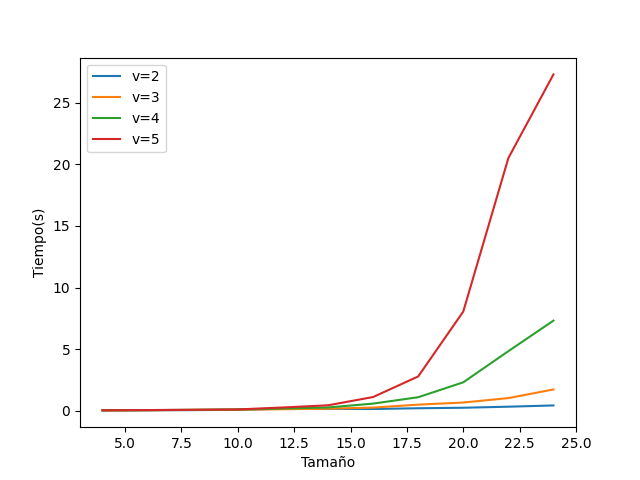
\includegraphics[width=\linewidth]{./images/Chapter-3/p-bp-8-24}
		\caption{BP}
	\end{subfigure}
	\begin{subfigure}{.49\linewidth}
		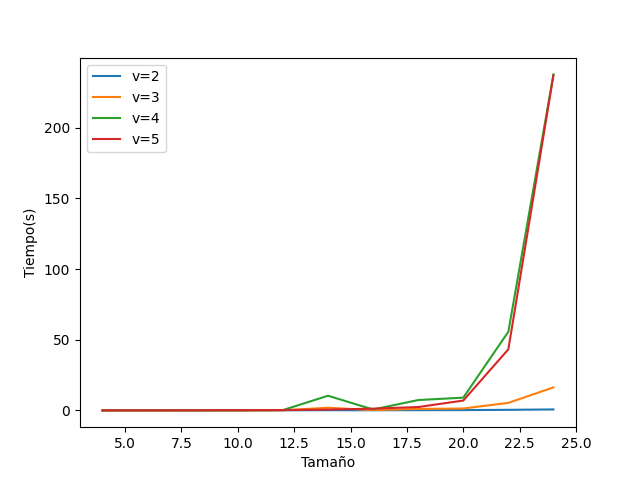
\includegraphics[width=\linewidth]{./images/Chapter-3/p-ve-8-24}
		\caption{VE}
	\end{subfigure}
	\caption{Comparación entre los algoritmos de propagación de creencias y eliminación de variables}
	\label{fig:p-24}
\end{figure}

\begin{figure}[h!]
	\centering
	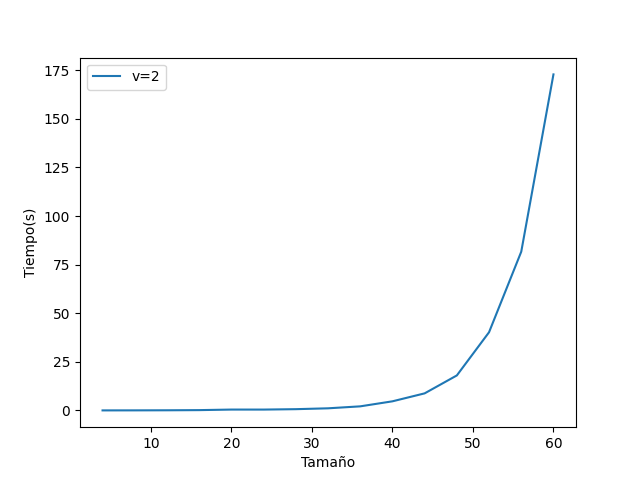
\includegraphics[width=0.5\linewidth]{./images/Chapter-3/p-bp-8-60}
	\caption{Comportamiento del algoritmo de propagación de creencias para modelos con sólo variables binarias}
	\label{fig:p-bp-8-60}
\end{figure}

Los contrafactuales resultaron ser viables en redes más pequeñas que las de las predicciones e intervenciones, pues el método de las redes gemelas transforma la red en una de casi el doble de su tamaño y realiza inferencia sobre ella. En la Figura \ref{fig:c-8-20} se muestra el comportamiento de los contrafactuales en dependencia del algoritmo que se use durante la fase de inferencia bayesiana en modelos con solo variables binarias.

\begin{figure}[h!]
	\centering
	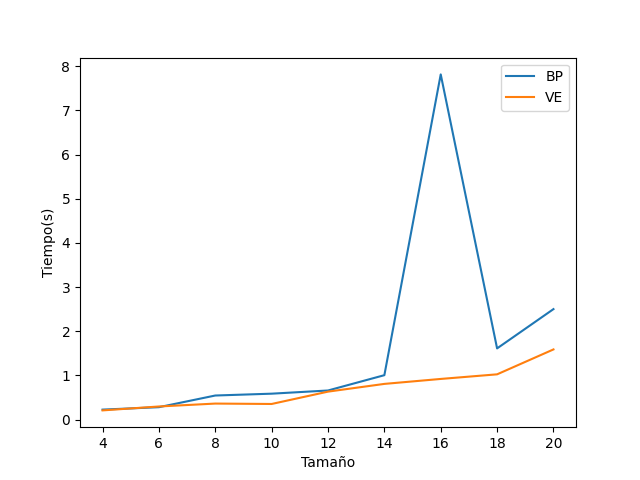
\includegraphics[width=0.5\linewidth]{./images/Chapter-3/c-8-20}
	\caption{propagación de creencias vs eliminación de variables en contrafactuales}
	\label{fig:c-8-20}
\end{figure}




\section{Interfaz de usuario}
La interfaz de usuario está concebida para facilitar el uso de la inferencia causal en problemas que lo requieran, abstrayendo al usuario del ambiente de la programación. Se brinda al usuario la posibilidad de crear, editar, cargar y guardar modelos estructurales causales. Además es posible visualizar el grafo causal asociado. Se brindan 5 modalidades de inferencia causal: predicción, intervención, contrafactual, atribución y mediación. Para cada tipo de inferencia se provee un formulario donde el usuario especifica los parámetros de la consulta a realizar. Para asegurar que la entrada provista por los usuarios al programa es la correcta, en todos los formularios existen métodos de validación que notifican al usuario en caso de que la entrada sea incorrecta.

La interfaz visual fue desarrollada con la librería \textbf{kivy}\cite{kivyDocs}. Entre sus principales características se encuentran que es de código abierto, multiplataforma y eficiente. Permite la creación de aplicaciones de manera rápida y a diferencia de otras librerías para interfaces visuales como PyQt, ofrece una sintaxis más elegante, al estilo de Python.

Para la visualización de los grafos causales se utilizaron dos librerías: \textbf{pydot}\cite{pydotDocs} y \textbf{networkx}\cite{networkxDocs}. Ello se debe a que en algunas arquitecturas de sistemas operativos la primera, que es la preferida, requiere de la instalación de dependencias adicionales, y no se desea que esa tarea recaiga en manos del usuario. Por ello cuando se solicita la imagen de un grafo causal, se da prioridad a \textit{pydot}, y en caso de que no sea posible utilizarla, se usa la segunda, que es más flexible.

Por último, para el proceso de empaquetado del software se utilizó \textbf{PyInstaller}\cite{PyInstaller}. Esta librería agrupa el código y las dependencias en un paquete que puede ser usado en otras computadoras sin la necesidad de instalar un intérprete de Python ni las dependencias, siempre y cuando sea en un sistema operativo similar a donde se construyo el paquete.

\begin{figure}
	\centering
	\begin{subfigure}{\linewidth}
		\centering
		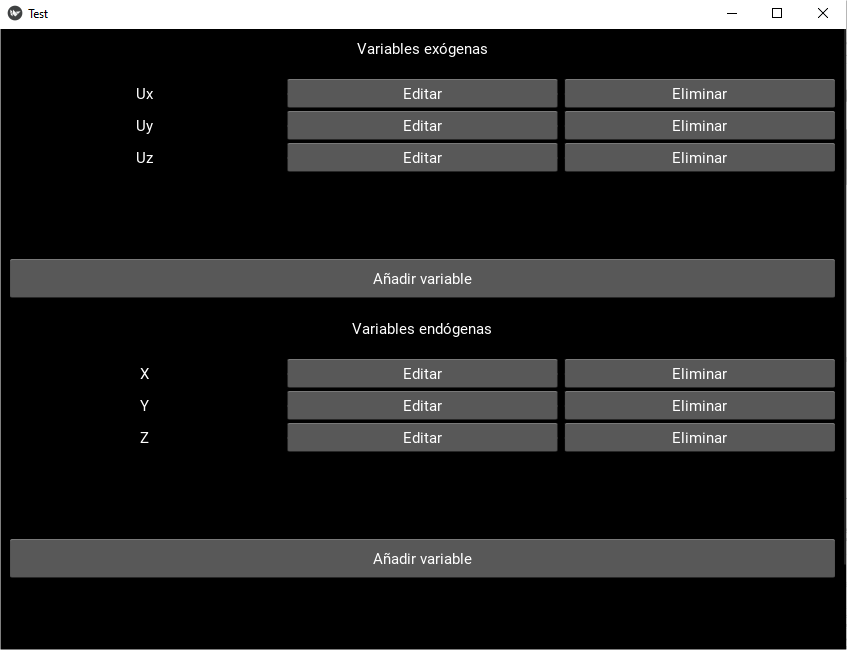
\includegraphics[width=300px, height=280px]{./images/Chapter-3/create-model}
		\caption{Ventana de creación de un modelo causal estructural}
		\label{fig:create-model}
	\end{subfigure}
	\begin{subfigure}{\linewidth}
		\centering
		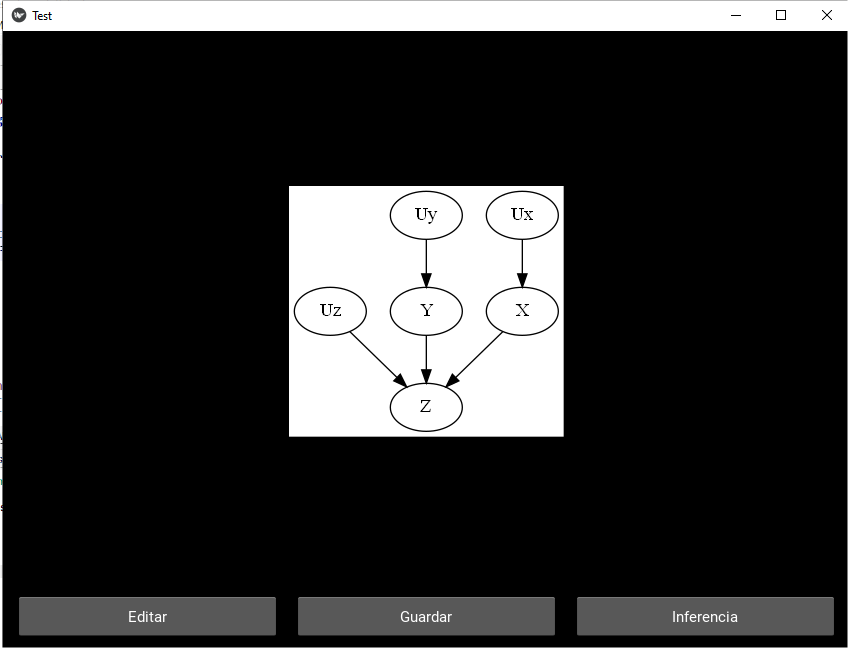
\includegraphics[width=300px, height=280px]{./images/Chapter-3/model-view}
		\caption{Ventana principal del modelo}
		\label{fig:model-view}
	\end{subfigure}
\end{figure}

\begin{figure}
	\begin{subfigure}{\linewidth}
		\centering
		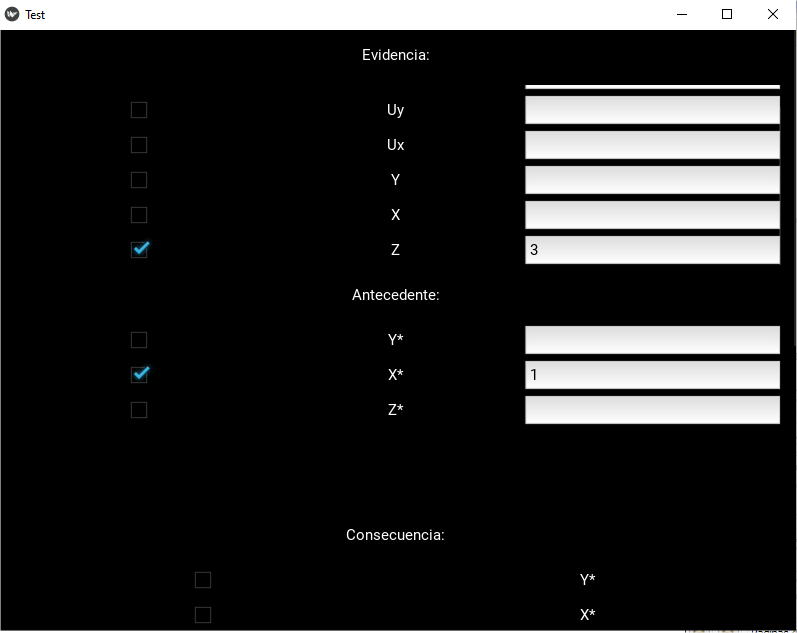
\includegraphics[width=300px, height=280px]{./images/Chapter-3/counterfactual(1)}
		\subcaption{}
		\label{fig:counterfactual-1}
	\end{subfigure}
	\begin{subfigure}{\linewidth}
		\centering
		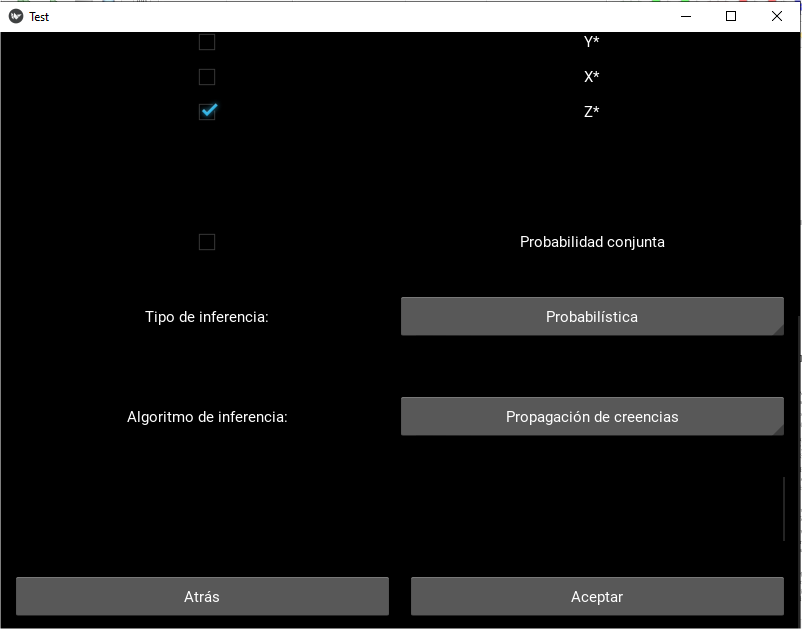
\includegraphics[width=300px, height=280px]{./images/Chapter-3/counterfactual(2)}
		\subcaption{}
		\label{fig:counterfactual-2}
	\end{subfigure}
	\subcaption{Formulario para calcular un contrafactual}
	\label{fig:counterfactual}
\end{figure}

\begin{figure}
	\centering
	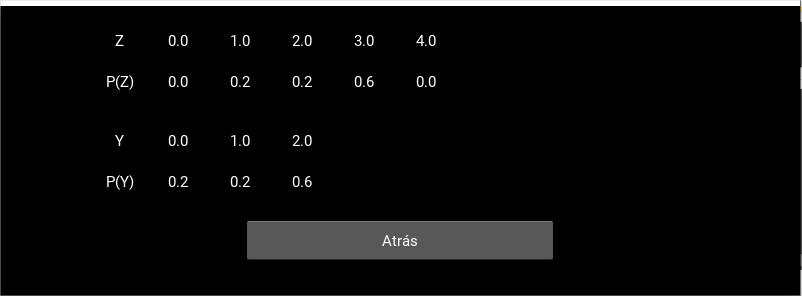
\includegraphics[width=300px, height=280px]{./images/Chapter-3/intervention-result}
	\caption{Resultados de una intervención}
	\label{fig:intervention}
\end{figure}
	\chapter{Detalles de implementación}\label{cap:implementation_details}

Con el objetivo de garantizar que el lector esté más acorde con la tecnología usada para la implementación, las razones de esa elección, la forma de desplegar el sistema y demás aspectos relacionados con la parte tecnológica se expone esta capítulo.

A día de hoy se cuenta con muchas herramientas para desarrollar un software de este tipo. En esta ocasión se escogió una tecnología que ha alcanzado bastante auge en los últimos años. En las secciones siguientes se hará alusión a la misma así como al lenguaje empleado para el desarrollo.

\section{Tecnologías}
Para este proyecto se utilizó el lenguaje TypeScript, auxiliándonos de NestJS (framework de NodeJS).

\label{lenguage}
\cite{wiki_ts}
TypeScript(TS) es un lenguaje de programación libre y de código abierto desarrollado y mantenido por Microsoft. Es un superconjunto de JavaScript(JS), que esencialmente añade tipos estáticos y objetos basados en clases. Anders Hejlsberg, diseñador de C\# y creador de Delphi y Turbo Pascal, se considera el desarrollador del lenguaje. TS es usado para desarrollar aplicaciones JS que se ejecutarán tanto en el lado del cliente como del servidor. El lenguaje extiende la sintaxis de JS, por tanto cualquier código JS existente debería  funcionar sin problemas. Está pensado para grandes proyectos, los cuáles a través de un compilador de TS se traducen a código JS original. TS soporta ficheros de definición que contengan información sobre los tipos de librerías JS existentes; esto permite a otros programas usar los valores definidos en los ficheros como si fueran entidades TS de tipado estático. El compilador de TS está escrito asimismo en TS. 

El lenguaje fue publicado en octubre de 2012 , después de dos años de desarrollo por parte de la compañía y desde esa fecha ha tenido en general, buena aceptación por parte de todos, lo que le mereció el mérito en 2020 como segundo lenguaje de programción más amado según la encuesta de Stack Overflow\cite{stack_overflow} 2020 Develop Survey.

\cite{nestjs_doc}
NestJS es un framework para construir eficientes y escalables aplicaciones del lado del servidor utilizando NodeJS. Posee soporte tanto para JS como para TS y combina elementos de Programación Orientada a Objetos (OOP, por sus siglas en inglés), Programación Funcional y Programación Funcional Reactiva. Nest posee un robusto framework HTTP basado en \textit{Express} (definido por defecto) y opcionalmente se puede configurar además el uso \textit{Fastify} como alternativa a \textit{Express}.

Ofrece un nivel de abstracción superior al que normalmente encontramos en los demás frameworks de Node(Express/Fastify), pero también expone sus APIs directamente al desarrollador. Esto le ofrece a los programadores la libertad de emplear la mayoría de las aplicaciones de 3$^{ros}$ desarrolladas para esos otros ambientes.

En los últimos años gracias a Node, ha supuesto un cambio sustancial en el desarrollo de aplicaciones del lado del servidor, pero, por otra parte y a pesar de las bondades que ofrece, aún no presenta una solución efectiva al problema de arquitectura. 

Nest se presenta como solución a esto, ya que posee una estructura que induce desde el principio a la utilización de patrones arquitectónicos. La arquitectura de Nest es inspirada en Angular.

Fue desarrollado por Kamil Mysliwiec, desarrollador de Google; el lanzamiento de su versión 9 se realizó el 8 de Julio de 2022.


\section{Arquitectura}

El  sistema presentado encierra una gran lógica de negocio y encontrar una forma aceptada de representar el mismo puede resultar, en muchos casos, de gran dificultad.

Para asegurar el correcto diseño de la aplicación, su posible extensión y adición de nuevas features (características), se hizo neceario utilizar una arquitectura, quizá un poco compleja, pero que permitiera enfocar todos los casos de uso que puedan surgir. 

El diseño guiado por dominio (DDD por sus siglas en inglés) es un enfoque para el desarrollo de software con necesidades complejas, mediante una profunda conexión de la implementación con los conceptos del modelo y núcleo del negocio.\cite{ddd_wiki} 

Para el software que nos envuelve se emplea una arquitectura por capas (Layered Architecture), centrada en DDD. Este enfoque es, sin lugar a dudas, una de los más empleados hoy en día. Impone una jerarquía y un acceso restringido a cada una de las estructuras del código; dígase: dominio, aplicación, infraestructura y presentación; las cuáles se encargan de la separación de las responsabilidades, y por tanto de la gestión de elementos específicos.

\begin{itemize}
	\item Dominio: Gestiona todo lo referente a la lógica que involucra las entidades descritas en las secciones previas (\ref{sec:entities}). Es la capa fundamental dentro de DDD.
	\item Aplicación: Se encarga de manejar todos los casos de uso que relacionados con cada entidad. A modo de ejemplo, todo sistema cuenta con cuatro casos de uso básicos: crear, leer, eliminar y editar.
	\item Infraestructura: Maneja todo lo relacionado con el acceso a datos. Contiene los repositorios y por tanto define una especie de envoltura (wrapper) que evita que se acceda directamente a la base de datos.
	\item Presentación: Se encarga de exponer todos los puntos de acceso a la API (Application Program Interface) y de gestionar  los consumidores (consumers), que tienen la responsabilidad de la gestión de eventos internos y externos al sistema.
\end{itemize}

\begin{figure}[h]
	\centering
	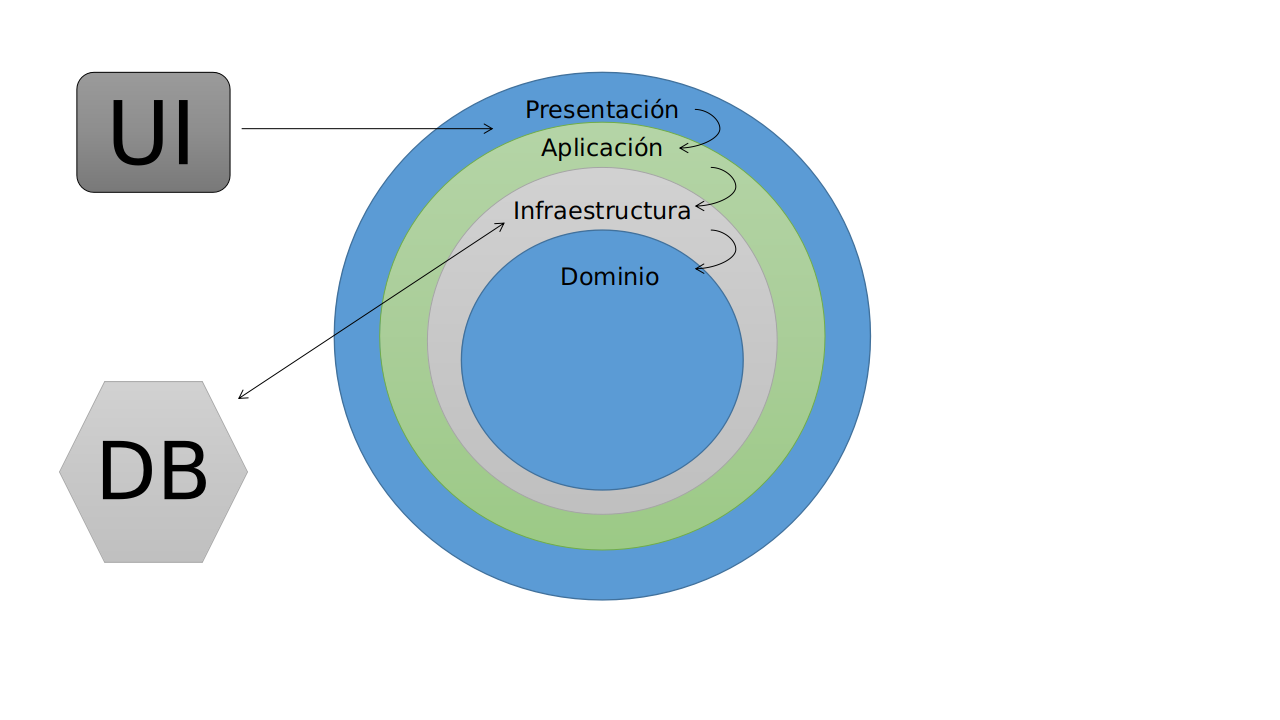
\includegraphics[width=0.75\linewidth]{images/Chapter 3/DDD}
	\caption{Domain Driven Design}
	\label{fig:ddd}
\end{figure}


Los principios \textit{SOLID} \cite{solid_medium} abordados por Robert C. Martin (autor de diversos libros como Clean Code y Clean Arquitecture) se interaron seguir a través de toda la implementación.


\section{Aplicación visual}

La idea detrás de la aplicación visual surge inspirada en un sistema desarrollado hace un par de años dentro de la facultad por un grupo de estudiantes y que se presentó como proyecto a la jornada científica de ese curso. \cite{horarios_fac}

Se ofrece un sistema desarrollado en VueJS y que pretende seguir las buenas prácticas de desarrollo de frontend. Está escrito en JavaScript. El sistema posee un conjunto de vistas dedicadas a manejar todas las tareas administrativas referentes al software; dígase: creación de profesores, grupos, semestres, asignaturas y demás cuestiones referentes al centro educacional. Solamente para el usuario con los permisos adecuados están habilitadas tales características, es decir, el usuario administrador es el único que puede realizar modificaciones internas dentro del sistema.

En la página principal se definen 5 tipos de filtros que hacen posible una rápida interacción. Estos filtros se presentan útiles en un gran número de escenarios. Se muestra además, en la misma página, la opción de descargar el horario, la cual esta habilitada para cualquier tipo de usuarios. El número que se presenta en la parte superior izquierda es referente a la felicidad del sistema, aspecto que fue abordado en las secciones previas a este capítulo. (\ref{sec:happiness})

En la visualización general del horario, cada grupo posee un color específico para que se haga más sencilla su lectura, el color es posible definirlo por el administrador del sistema a la hora de la creación del grupo, luego todos los turnos de clase que se asocien al mismo, se mostrarán de ese color.

\begin{figure}[h!]
	\centering
	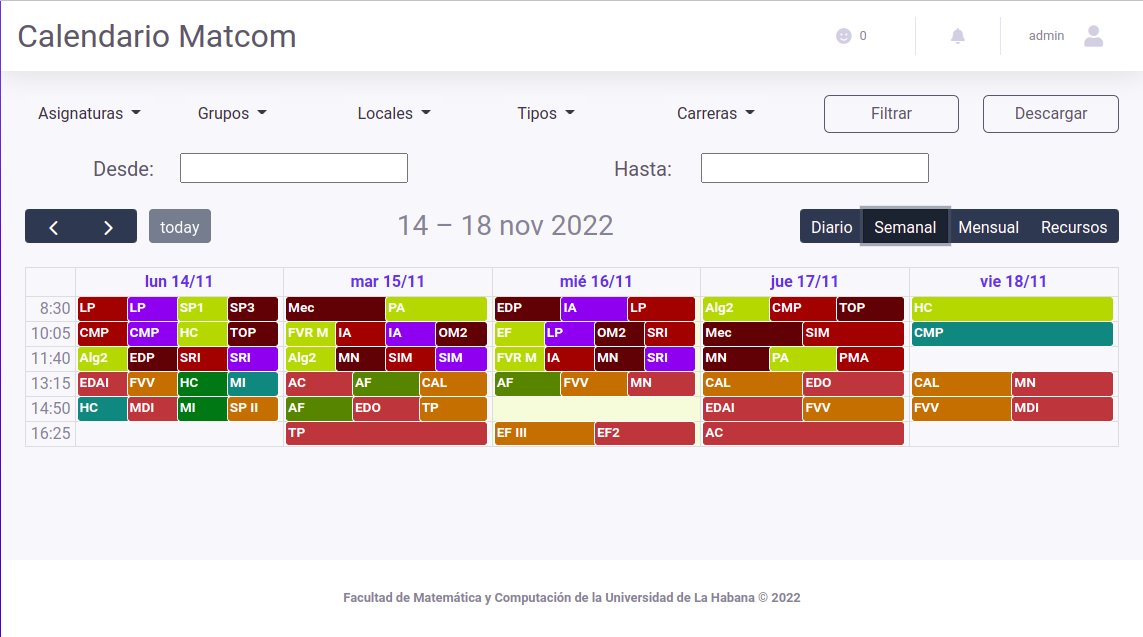
\includegraphics[width=0.95\linewidth]{images/Chapter 3/home}
	\caption{Vista por defecto del sistema.}
	\label{fig:home}
\end{figure}



En el manejo de la interfaz visual quizá resulte un poco llamativo para el administrador del sistema; que es el que tiene acceso a esas vistas; la creación, modificación y eliminación en serie que se muestra en cada \textit{modal} referente a los turnos de clases.  Este aspecto fue abordado con anterioridad, pero la acción que realiza es modificar todos los turnos que posean las mismas características del turno actual, es decir, que repitan el ciclo del horario para él.

Para cada turno visualizado es válido además modificarle la duración del mismo, esto se logra modificando el \textit{size} de este dentro del horario. Realizar esta acción es justo como modificarle el \textit{size} a cualquier otra ventana del sistema, lo que en esta ocasión es a la caja que describe el turno.

Haciendo clic encima del turno se obtine además una descripción detallada del mismo, así como las opciones para la edición y eliminación múltiple.

La vista de distribución por locales llama la atención y se presenta de gran importancia a la hora de considerar la usabilidad de la aplicación.

\begin{figure}[h!]
	\centering
	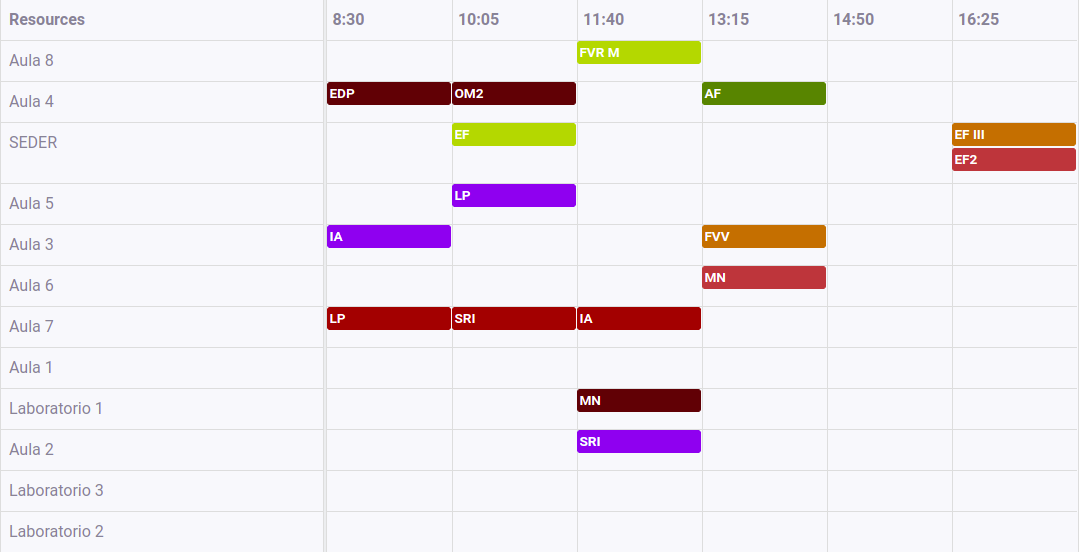
\includegraphics[width=0.95\linewidth]{images/Chapter 3/resource_distribution}
	\caption{Distribución por locales de los turnos de clase.}
	\label{fig:resource_distributions}
\end{figure}

\section{Autenticación}

La autenticación es una parte esencial en la mayoría de los sistemas y aplicaciones. Existen muchas formas y estrategias de manejar la misma. En el software que se presenta se pone en uso a través de un módulo independiente que posee todos los casos de uso y middlewares relacionados con tal aspecto. En esta ocasión el proceso se realiza por medio de JSON Web Token(JWT).

JWT es un estándar de internet propuesto para la creación de firmas y/o encriptación (opcional), cuyo contenido es enviado en forma de cadena de texto de backend a frontend (y viceversa), comunmente llamado \textit{token}.

\begin{figure}[h!]
	\centering
	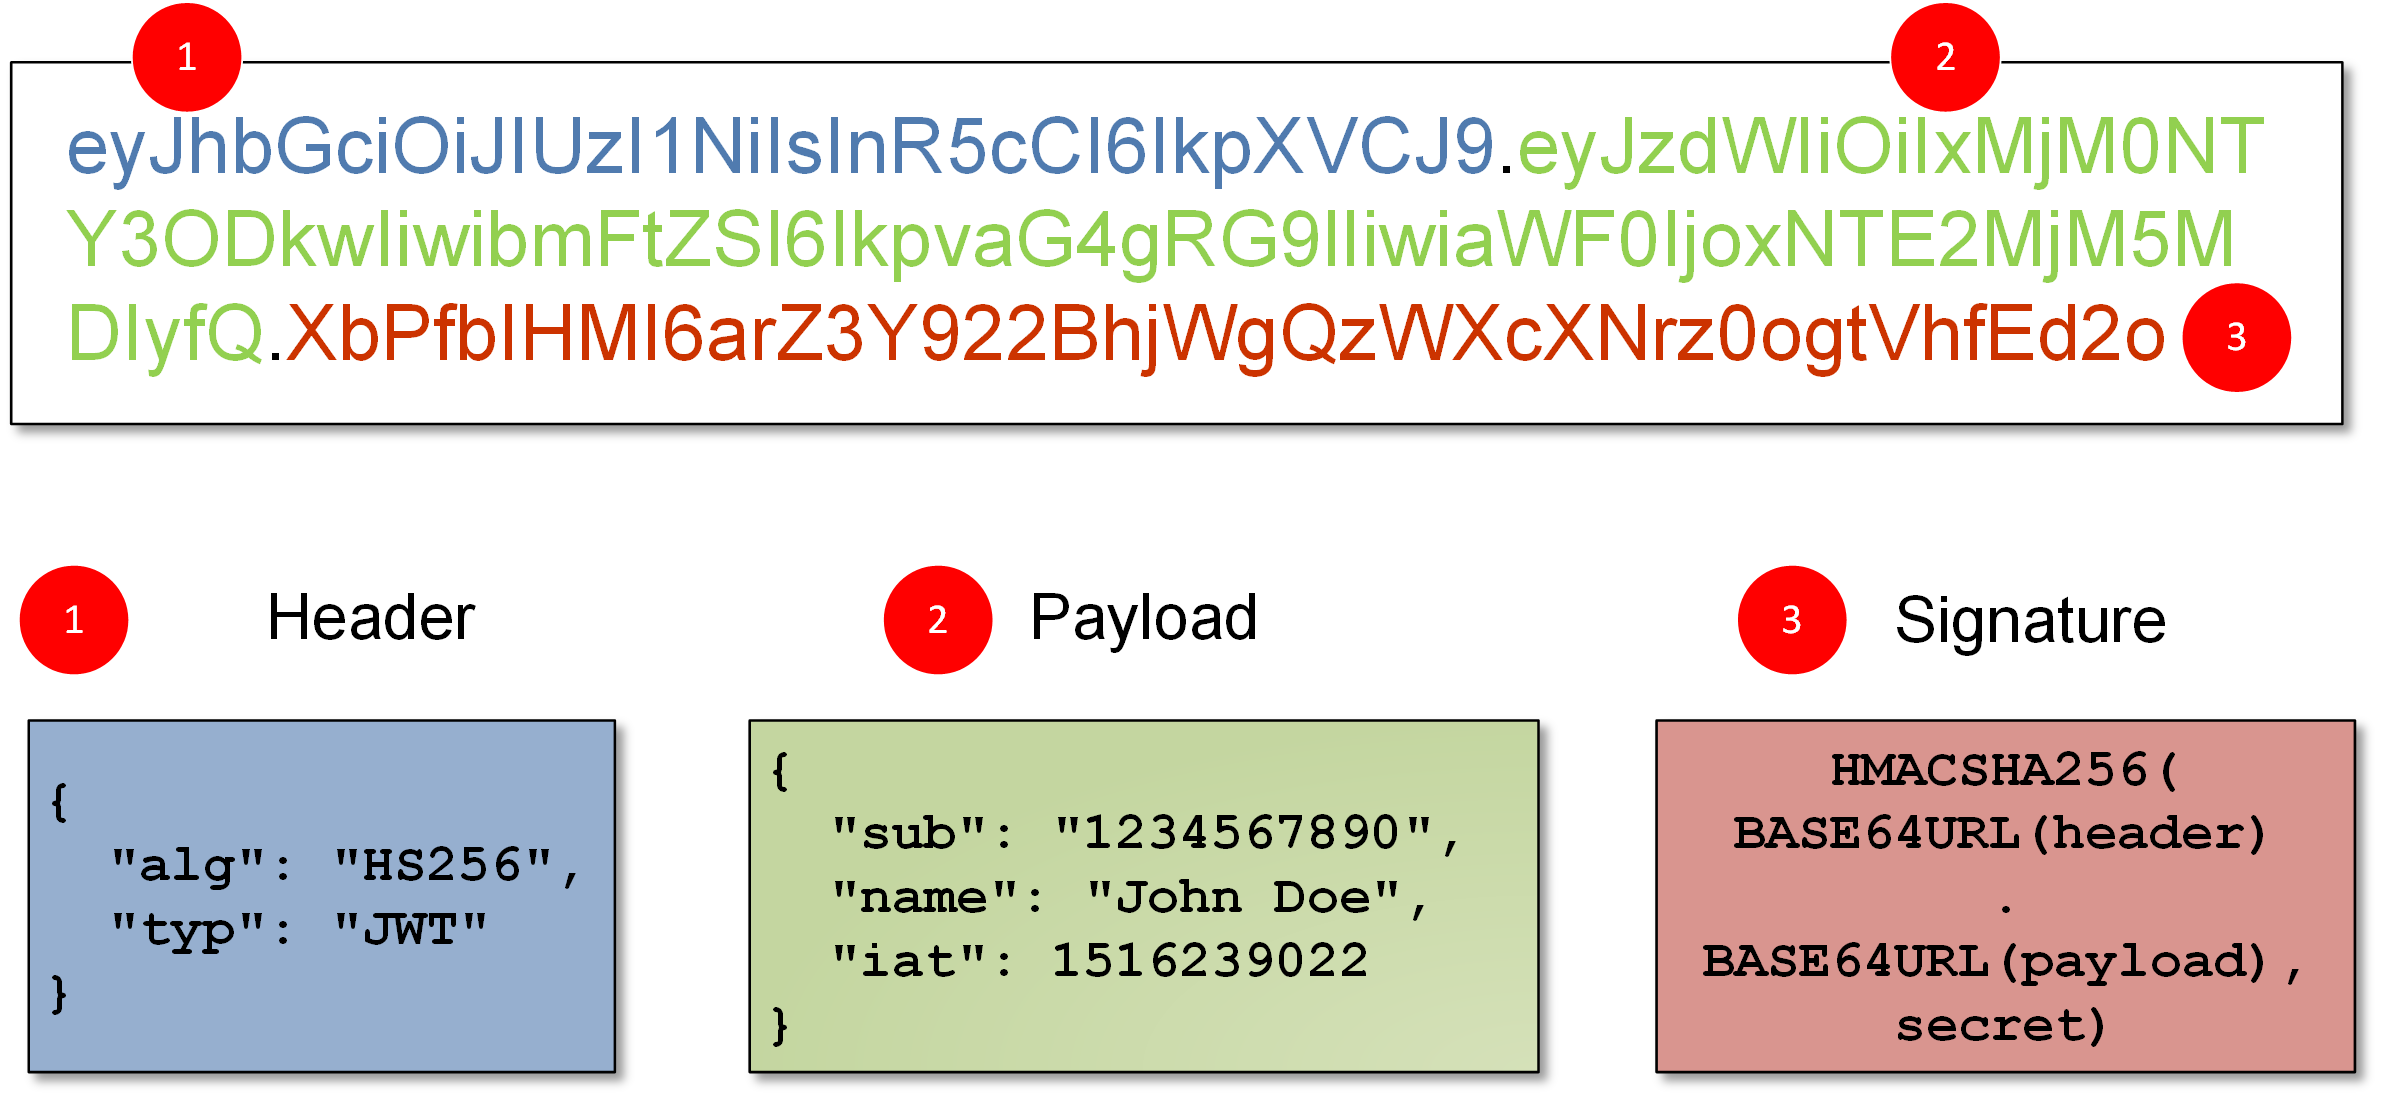
\includegraphics[width=0.95\linewidth]{images/Chapter 3/jwt1}
	\caption{Estructura del token \cite{jwt_image}}
	\label{fig:jwt}
\end{figure}

Cuando se recibe una petición de login por parte del cliente, el servidor se encarga de comprobar que las credenciales son correctas y la respuesta del login, es entre otras cosas, el token al que se hace referencia en el párrafo anterior. Supongamos después que se hace otra petición cliente-servidor y que el token se adjunta de forma apropiada en las cabeceras de la misma, cuando la petición arriba al punto adecuado, el servidor se encarga de ejecutar un \textit{middleware} (función intermedia) que procesa el token y verifica que sea el correcto, si todo este proceso se ejecuta sin mayores contratiempos, entonces en el request de la petición a través del campo user (request.user) se puede acceder al usuario que está intentado realizar la acción. En otro caso se responde con un estado 401 lo que indica que el usuario no esta autorizado al acceder al recurso que intenta solicitar. 

Todo este proceso antes descrito se realiza por medio de un paquete de terceros \textit{@nestjs/jwt} y además con la intervención de \textit{passport-jwt}



\section{Permisos y Usuarios}

En este sistema en particular los usuarios se clasifican en 2 grupos:

\begin{itemize}
	\item Los que solo pueden consultar el horario .
	\item Los que puede realizar acciones sobre algunas de sus entidades.
\end{itemize}

El primer grupo hace referencia a los usuario que solamente consultarán el sistema con el objetivo de estar al tanto de la información que se muestra en el mismo. Estos usuarios son considerados anónimos y por tanto solo podrán consumir los puntos de acceso que estén libres de permisos. Para ellos además se brindará la posibilidad de descargar el horario en formato Excel así como de estar al tanto de la felicidad del sistema.

El segundo grupo de usuario se separa, por otra parte, en dos conjuntos:

\begin{itemize}
	\item Profesores
	\item Usuarios administradores
\end{itemize}

A los profesores - previamente definidos por el administrador - se les dará la posibilidad de imponer sus propias restricciones (\ref{sec:restrictions}) sobre la distribución realizada e influir por en la felicidad final del sistema. Todas las demás utilidades están bloqueados para ellos.

Por otra parte, los administradores, son los que poseen todos los permisos; es decir, ellos tienen la potestad de modificar cualquier aspecto dentro del sistema; tanto de los turnos de clase como de las demás características relacionadas con la institución.

Los permisos son manejados por medio de un entero de 64 bits. Esto hace posible la optimización de espacio en la base de datos, así como la fácil representación de los mismos. Cada bit activo del número indica que el usuario \textit{X} puede realizar la acción correspondiente; luego para proceder al chequeo de estos, solo se hace necesario aplicar el operador binario \& (\ref{fig:and}) entre el entero que representa los permisos y el permiso en específico que se desea comprobar. Si el resultado de esta operación es mayor a 0, entonces el usuario puede completar la acción, en caso contrario se procede en consecuencia  y se responde negativamente al respecto.

\begin{figure}[h!]
	\centering
	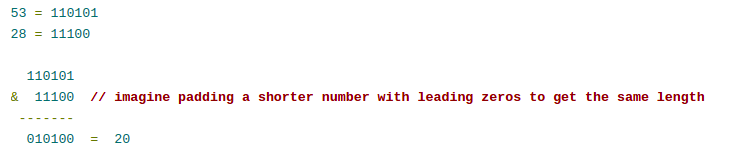
\includegraphics[width=0.95\linewidth]{images/Chapter 3/and}
	\caption{Operador \& entre dos números \cite{codeforces}}
	\label{fig:and}
\end{figure}

\noindent Luego activar un permiso para un usuario determinado no es más que: \\
\begin{equation}
	P \mid= (1 \ll p) \text{,}
\end{equation}

\noindent y para removerlo:\\
\begin{equation}
	\begin{split}	
		x & = \log_{2}(p \& -p) + 1  \\
		P & = P \& \sim(1 \ll (x - 1))
	\end{split}
\end{equation}

\noindent Donde se tiene que: \\
\begin{itemize}
	\item $P$: valor entero que representa los permisos que posee el usuario.
	\item $p$: permiso que se intenta adicionar o remover, según sea el caso.
\end{itemize}

Este enfoque ofrecido para los permisos, posee un inconveniente que no es muy difícil de notar: solamente se pueden representar 64 permisos en el sistema. En el software que se presenta, 64 permisos son más que suficientes para  gestionar todas las necesidades del mismo.

\section{Sistema de reportes}

Contar con una fácil distribución del contenido de manera offline, es un aspecto de notable importancia en muchos sistemas. En el que se propone, esta opción también se encuentra habilitada. 

Existe un módulo dedicado a cumplir esta tarea. La librería de NPM (Node Package Module) \texttt{excel4node}\cite{excel4node_npm}, es la encargada de gestionar e intervenir en todos los aspectos relacionados con la generación de un fichero en formato \textit{Excel} para asegurar cumplido el objetivo. Son innumerables las bondades que ofrece la misma, así como la facilidad para el trabajo con este tipo de ficheros, por tales motivos no trajo mayores dificultades considerar la utilización de esta en el desarrollo del software.

\section{Base de datos}

La base de datos que se utiliza para gestionar todo lo relacionado con la aplicación es \textit{PostgreSQL}; este es uno de los servidores de bases de datos más conocidos y utilizados a día de hoy. Está desarrollado bajo código abierto, razón por la que posee una gran comunidad que se encarga de trabajar en nuevas características constantemente. 

Existen varias razones que hacen que PostgreSQL resulte llamativo y que, por tanto, llevaron a su elección para este proyecto.
\begin{itemize}
	\item Multiplataforma: Se encuentra disponible en todas las versiones de los sistemas operativos Windows, Linux y Mac.
	\item Alto volumen: Ofrece un gran rendimiento cuando se hace necesario trabajar con grades volúmenes de información. Gracias al método de \textit{Control de Concurrencias Multiversión} se consigue un mejor performance cuando hay muchos movimientos dentro de la base de datos.
	\item Facilidad de manejo.
	\item Seguridad de la información: Hot-Standby es una de las cualidades más interesantes de Postgres. Hot-Standby permite que los usuarios puedan acceder a las tablas en modo lectura mientras que se realizan los procesos de backup o mantenimiento.
	\item \texttt{Tipos de datos}: Tiene soporte para tipos de datos avanzados tales como: arrays, hstore y tipos definidos por el usuario.
\end{itemize}

\section{Docker} 


Docker es una plataforma de código abierto para el desarrollo, manejo y ejecución de aplicaciones. Ofrece la ventaja de separar las aplicaciones de la infraestructura, por tal razón el despliegue de los sistemas se puede realizar relativamente rápido. Con el uso de docker  la infraestructura se maneja de la misma manera que se hace con las aplicaciones. Hablando de ventajas, las metodologías de docker para despliegue, integración y pruebas hacen que se reduzca significativamente el tiempo entre la escritura del código y el despliegue en producción del mismo. Además provee la habilidad de empaquetar y correr una aplicación en un ambiente aislado llamado \textit{contenedor}. Debido a este aislamiento y a la seguridad que ofrece se permite ejecutar varias aplicaciones simultaneamente en un servidor. Los contenedores son ligeros y contienen todo lo necesario para correr la aplicación, de esta forma, no es necesario preocuparse por lo que el serividor necesite instalar para su funcionamiento. Se puede compartir un contenedor mientras se está desarrollando  un proyecto y se garantiza que culaquiera que ejecute el mismo contenedor contendrá exactamente el mismo ambiente de trabajo que el desarrollador inicial.\cite{docker_dfn}

El sistema que se ofrece se encuentra desarrollado completamente sobre docker, tanto el frontend (que se despliega sobre nginx) como el backend (que se despliega sobre node). Esta integración hará que resulte de gran facilidad la instalación del software sobre cualquier red y que por tanto su pase a producción se realice sin mayores complicaciones. 

Las imágenes manejadas dentro del sistema están descritas en el siguiente enumerado; todas están disponibles en \href{https://hub.docker.com/}{\textit{Docker Hub}}:
\begin{itemize}
	\item node:16-alpine
	\item postgis/postgis:13-3.1-alpine
	\item adminer:latest
	\item nginx
\end{itemize}

El uso de ngnix será descrito en la siguiente sección.

\subsection{NGINX}

Nginx server es un servidor web gratuito y de código abierto. Se ejecuta en sistemas operativos Linux/Unix de 64 bits y es ampliamente utilizado para sitios web de alto rendimiento debido a su arquitectura liviana en comparación con otros servidores de la misma clase.

La herramienta fue incluida en este proyecto por medio de una imagen de Docker; e hizo posible que el frontend se desplegara a través de un servidor que se encargara de gestionar todos los temas de performance y manejo de peticiones.

Nginx fue lanzado oficialmente en octubre del 2004. El creador del software, Igor Sysoev, comenzó su proyecto en el 2002 como un intento de solucionar el problema C10k (reto de gestionar diez mil conexiones al mismo tiempo). Hoy en día, los servidores web tienen que manejar un número aún mas grande de conexiones. Por esa razón, Nginx ofrece una arquitectura asíncrona y controlada por eventos, característica que hace de él uno de los servidores más confiables para la velocidad y la escalabilidad. Muchos sitios web de alto tráfico usan el servicio, algunos de estos gigantes del internet son Google, Netflix, Adobe, Cloudflare, WordPress.com por solo mencionar algunos. \cite{nginx}



	\begin{conclusions}
%	Se realizó un recorrido general por la historia del desarrollo matemático y filosófico de la causalidad. El problema recayó primeramente en manos de los filósofos y comenzó a despertar el interés de algunos matemáticos a principios de la época moderna. Sin embargo fue abandonado tempranamente dado que estos desviaron su atención hacia la estadística, área de la matemática que también daba sus primeros pasos por aquel entonces. La evasión de la causalidad por parte de los estadísticos condujo al surgimiento de numerosas paradojas y problemas intratables por la falta de las herramientas adecuadas para encararlos, herramientas que no podía proporcionar la visión frecuentista de la estadística. La historia de la concepción matemática de la causalidad tiene su punto de inflexión con la publicación de Sewall Wright de los diagramas de caminos. Posteriormente comenzaron a desarrollarse diversas teorías y modelos que explican la causalidad, con Reichenbach, Suppes, Granger y Pearl entre sus principales exponentes.
%	
%	Se expusieron los desarrollos de Judea Pearl en la teoría de la causalidad y los modelos gráficos probabilistas. Se repasó la teoría de la independencia condicional como base para el desarrollo de los modelos gráficos probabilistas. Se presentaron las redes bayesianas como un primer modelo capaz de realizar predicciones en las variables a partir de observaciones. Posteriormente se introdujo el modelo causal estructural de Pearl como modelo gráfico probabilista capaz de representar explícitamente las relaciones de causalidad entre variables y su relación con las redes bayesianas. A continuación se pasó a introducir las distintas modalidades de inferencia causal propias de un SCM. Primeramente se formalizó el concepto de intervención, definiendo el operador \textit{do} y resaltando sus diferencias con la observación pasiva. A continuación se vieron los principales métodos de inferencia causal para el cálculo de intervenciones: el criterio de la puerta trasera, el criterio de la puerta principal, el cálculo-do y la inferencia bayesiana. Luego se expuso la teoría relacionada con los contrafactuales, sus variantes determinista y no determinista y los principales métodos para calcularlos, haciendo especial hincapié en el método de las redes gemelas. Por último se expusieron dos aplicaciones de las intervenciones y los contrafactuales conocidos como atribución y mediación. La primera permite explicar el comportamiento de una variable a partir del de otras y la segunda, el análisis del efecto que ejerce una variable sobre otra a través de un mediador.
%	
%	Se desarrolló una implementación de los algoritmos de inferencia causal, utilizando la idea de la cirugía en el grafo para intervenir el modelo y el método de las redes gemelas para calcular los contrafactuales, conjuntamente con la idea de transformar el modelo a una red bayesiana para aplicar inferencia bayesiana y obtener la respuesta a la consulta deseada.
%	
%	Los algoritmos de inferencia causal se comportaron satisfactoriamente para modelos cuyos grafos son esparcidos y las variables toman una cantidad relativamente pequeña de valores. Sin embargo, cuando el número de nodos, estados y aristas del grafo causal crece notablemente, el tiempo de ejecución se ve comprometido, especialmente en el caso de los contrafactuales, en los cuales la inferencia es aplicada en un grafo que en el caso peor ocupa el doble de tamaño que el grafo original. La técnica de mezcla de nodos resultó ser útil para disminuir el costo computacional de calcular los contrafactuales.
%	
%	Además se desarrolló una interfaz visual destinada a usuarios no expertos en programación para la resolución de problemas de naturaleza causal.
%	
%	Por último se mostraron algunas aplicaciones de la teoría de la causalidad en las que puede ser utilizado el programa implementado.
%	
%	La causalidad ha demostrado ser una herramienta útil para complementar el procesamiento estadístico de los datos. Su uso permite la modelación y el entendimiento de procesos que la asociación no captura. Simular intervenciones a partir de datos recopilados, en vez de llevar a cabo la intervención en la práctica, permite no solo el ahorro de recursos, sino también conocer el resultado de intervenciones que serían imposibles o inviables de determinar experimentalmente.
%	
%	Para concluir, se debe resaltar que la simulación del pensamiento causal nos colocará un paso más cerca de simular el pensamiento humano. Dotar de razonamiento causal a las máquinas permitirá que estas adquieran capacidades distintivas del ser humano, como son planear acciones con antelación o aprender de los propios errores. Conforme surjan nuevas teorías que mejoren, extiendan y complementen las actuales y se desarrollen modelos más completos y realistas capaces de razonar casualmente, seremos capaces no solo de automatizar tareas complejas, sino además de entendernos mejor a nosotros mismos.	
\end{conclusions}
	
	\backmatter
	\renewcommand{\bibname}{Referencias}

\bibliographystyle{unsrt}
\bibliography{References/references}

\end{document}
